% Options for packages loaded elsewhere
\PassOptionsToPackage{unicode}{hyperref}
\PassOptionsToPackage{hyphens}{url}
\PassOptionsToPackage{dvipsnames,svgnames,x11names}{xcolor}
%
\documentclass[
  letterpaper,
  DIV=11,
  numbers=noendperiod]{scrartcl}

\usepackage{amsmath,amssymb}
\usepackage{iftex}
\ifPDFTeX
  \usepackage[T1]{fontenc}
  \usepackage[utf8]{inputenc}
  \usepackage{textcomp} % provide euro and other symbols
\else % if luatex or xetex
  \usepackage{unicode-math}
  \defaultfontfeatures{Scale=MatchLowercase}
  \defaultfontfeatures[\rmfamily]{Ligatures=TeX,Scale=1}
\fi
\usepackage{lmodern}
\ifPDFTeX\else  
    % xetex/luatex font selection
\fi
% Use upquote if available, for straight quotes in verbatim environments
\IfFileExists{upquote.sty}{\usepackage{upquote}}{}
\IfFileExists{microtype.sty}{% use microtype if available
  \usepackage[]{microtype}
  \UseMicrotypeSet[protrusion]{basicmath} % disable protrusion for tt fonts
}{}
\makeatletter
\@ifundefined{KOMAClassName}{% if non-KOMA class
  \IfFileExists{parskip.sty}{%
    \usepackage{parskip}
  }{% else
    \setlength{\parindent}{0pt}
    \setlength{\parskip}{6pt plus 2pt minus 1pt}}
}{% if KOMA class
  \KOMAoptions{parskip=half}}
\makeatother
\usepackage{xcolor}
\setlength{\emergencystretch}{3em} % prevent overfull lines
\setcounter{secnumdepth}{-\maxdimen} % remove section numbering
% Make \paragraph and \subparagraph free-standing
\makeatletter
\ifx\paragraph\undefined\else
  \let\oldparagraph\paragraph
  \renewcommand{\paragraph}{
    \@ifstar
      \xxxParagraphStar
      \xxxParagraphNoStar
  }
  \newcommand{\xxxParagraphStar}[1]{\oldparagraph*{#1}\mbox{}}
  \newcommand{\xxxParagraphNoStar}[1]{\oldparagraph{#1}\mbox{}}
\fi
\ifx\subparagraph\undefined\else
  \let\oldsubparagraph\subparagraph
  \renewcommand{\subparagraph}{
    \@ifstar
      \xxxSubParagraphStar
      \xxxSubParagraphNoStar
  }
  \newcommand{\xxxSubParagraphStar}[1]{\oldsubparagraph*{#1}\mbox{}}
  \newcommand{\xxxSubParagraphNoStar}[1]{\oldsubparagraph{#1}\mbox{}}
\fi
\makeatother

\usepackage{color}
\usepackage{fancyvrb}
\newcommand{\VerbBar}{|}
\newcommand{\VERB}{\Verb[commandchars=\\\{\}]}
\DefineVerbatimEnvironment{Highlighting}{Verbatim}{commandchars=\\\{\}}
% Add ',fontsize=\small' for more characters per line
\usepackage{framed}
\definecolor{shadecolor}{RGB}{241,243,245}
\newenvironment{Shaded}{\begin{snugshade}}{\end{snugshade}}
\newcommand{\AlertTok}[1]{\textcolor[rgb]{0.68,0.00,0.00}{#1}}
\newcommand{\AnnotationTok}[1]{\textcolor[rgb]{0.37,0.37,0.37}{#1}}
\newcommand{\AttributeTok}[1]{\textcolor[rgb]{0.40,0.45,0.13}{#1}}
\newcommand{\BaseNTok}[1]{\textcolor[rgb]{0.68,0.00,0.00}{#1}}
\newcommand{\BuiltInTok}[1]{\textcolor[rgb]{0.00,0.23,0.31}{#1}}
\newcommand{\CharTok}[1]{\textcolor[rgb]{0.13,0.47,0.30}{#1}}
\newcommand{\CommentTok}[1]{\textcolor[rgb]{0.37,0.37,0.37}{#1}}
\newcommand{\CommentVarTok}[1]{\textcolor[rgb]{0.37,0.37,0.37}{\textit{#1}}}
\newcommand{\ConstantTok}[1]{\textcolor[rgb]{0.56,0.35,0.01}{#1}}
\newcommand{\ControlFlowTok}[1]{\textcolor[rgb]{0.00,0.23,0.31}{\textbf{#1}}}
\newcommand{\DataTypeTok}[1]{\textcolor[rgb]{0.68,0.00,0.00}{#1}}
\newcommand{\DecValTok}[1]{\textcolor[rgb]{0.68,0.00,0.00}{#1}}
\newcommand{\DocumentationTok}[1]{\textcolor[rgb]{0.37,0.37,0.37}{\textit{#1}}}
\newcommand{\ErrorTok}[1]{\textcolor[rgb]{0.68,0.00,0.00}{#1}}
\newcommand{\ExtensionTok}[1]{\textcolor[rgb]{0.00,0.23,0.31}{#1}}
\newcommand{\FloatTok}[1]{\textcolor[rgb]{0.68,0.00,0.00}{#1}}
\newcommand{\FunctionTok}[1]{\textcolor[rgb]{0.28,0.35,0.67}{#1}}
\newcommand{\ImportTok}[1]{\textcolor[rgb]{0.00,0.46,0.62}{#1}}
\newcommand{\InformationTok}[1]{\textcolor[rgb]{0.37,0.37,0.37}{#1}}
\newcommand{\KeywordTok}[1]{\textcolor[rgb]{0.00,0.23,0.31}{\textbf{#1}}}
\newcommand{\NormalTok}[1]{\textcolor[rgb]{0.00,0.23,0.31}{#1}}
\newcommand{\OperatorTok}[1]{\textcolor[rgb]{0.37,0.37,0.37}{#1}}
\newcommand{\OtherTok}[1]{\textcolor[rgb]{0.00,0.23,0.31}{#1}}
\newcommand{\PreprocessorTok}[1]{\textcolor[rgb]{0.68,0.00,0.00}{#1}}
\newcommand{\RegionMarkerTok}[1]{\textcolor[rgb]{0.00,0.23,0.31}{#1}}
\newcommand{\SpecialCharTok}[1]{\textcolor[rgb]{0.37,0.37,0.37}{#1}}
\newcommand{\SpecialStringTok}[1]{\textcolor[rgb]{0.13,0.47,0.30}{#1}}
\newcommand{\StringTok}[1]{\textcolor[rgb]{0.13,0.47,0.30}{#1}}
\newcommand{\VariableTok}[1]{\textcolor[rgb]{0.07,0.07,0.07}{#1}}
\newcommand{\VerbatimStringTok}[1]{\textcolor[rgb]{0.13,0.47,0.30}{#1}}
\newcommand{\WarningTok}[1]{\textcolor[rgb]{0.37,0.37,0.37}{\textit{#1}}}

\providecommand{\tightlist}{%
  \setlength{\itemsep}{0pt}\setlength{\parskip}{0pt}}\usepackage{longtable,booktabs,array}
\usepackage{calc} % for calculating minipage widths
% Correct order of tables after \paragraph or \subparagraph
\usepackage{etoolbox}
\makeatletter
\patchcmd\longtable{\par}{\if@noskipsec\mbox{}\fi\par}{}{}
\makeatother
% Allow footnotes in longtable head/foot
\IfFileExists{footnotehyper.sty}{\usepackage{footnotehyper}}{\usepackage{footnote}}
\makesavenoteenv{longtable}
\usepackage{graphicx}
\makeatletter
\def\maxwidth{\ifdim\Gin@nat@width>\linewidth\linewidth\else\Gin@nat@width\fi}
\def\maxheight{\ifdim\Gin@nat@height>\textheight\textheight\else\Gin@nat@height\fi}
\makeatother
% Scale images if necessary, so that they will not overflow the page
% margins by default, and it is still possible to overwrite the defaults
% using explicit options in \includegraphics[width, height, ...]{}
\setkeys{Gin}{width=\maxwidth,height=\maxheight,keepaspectratio}
% Set default figure placement to htbp
\makeatletter
\def\fps@figure{htbp}
\makeatother

\usepackage{booktabs}
\usepackage{longtable}
\usepackage{array}
\usepackage{multirow}
\usepackage{wrapfig}
\usepackage{float}
\usepackage{colortbl}
\usepackage{pdflscape}
\usepackage{tabu}
\usepackage{threeparttable}
\usepackage{threeparttablex}
\usepackage[normalem]{ulem}
\usepackage{makecell}
\usepackage{xcolor}
\KOMAoption{captions}{tableheading}
\makeatletter
\@ifpackageloaded{tcolorbox}{}{\usepackage[skins,breakable]{tcolorbox}}
\@ifpackageloaded{fontawesome5}{}{\usepackage{fontawesome5}}
\definecolor{quarto-callout-color}{HTML}{909090}
\definecolor{quarto-callout-note-color}{HTML}{0758E5}
\definecolor{quarto-callout-important-color}{HTML}{CC1914}
\definecolor{quarto-callout-warning-color}{HTML}{EB9113}
\definecolor{quarto-callout-tip-color}{HTML}{00A047}
\definecolor{quarto-callout-caution-color}{HTML}{FC5300}
\definecolor{quarto-callout-color-frame}{HTML}{acacac}
\definecolor{quarto-callout-note-color-frame}{HTML}{4582ec}
\definecolor{quarto-callout-important-color-frame}{HTML}{d9534f}
\definecolor{quarto-callout-warning-color-frame}{HTML}{f0ad4e}
\definecolor{quarto-callout-tip-color-frame}{HTML}{02b875}
\definecolor{quarto-callout-caution-color-frame}{HTML}{fd7e14}
\makeatother
\makeatletter
\@ifpackageloaded{caption}{}{\usepackage{caption}}
\AtBeginDocument{%
\ifdefined\contentsname
  \renewcommand*\contentsname{Table of contents}
\else
  \newcommand\contentsname{Table of contents}
\fi
\ifdefined\listfigurename
  \renewcommand*\listfigurename{List of Figures}
\else
  \newcommand\listfigurename{List of Figures}
\fi
\ifdefined\listtablename
  \renewcommand*\listtablename{List of Tables}
\else
  \newcommand\listtablename{List of Tables}
\fi
\ifdefined\figurename
  \renewcommand*\figurename{Figure}
\else
  \newcommand\figurename{Figure}
\fi
\ifdefined\tablename
  \renewcommand*\tablename{Table}
\else
  \newcommand\tablename{Table}
\fi
}
\@ifpackageloaded{float}{}{\usepackage{float}}
\floatstyle{ruled}
\@ifundefined{c@chapter}{\newfloat{codelisting}{h}{lop}}{\newfloat{codelisting}{h}{lop}[chapter]}
\floatname{codelisting}{Listing}
\newcommand*\listoflistings{\listof{codelisting}{List of Listings}}
\makeatother
\makeatletter
\makeatother
\makeatletter
\@ifpackageloaded{caption}{}{\usepackage{caption}}
\@ifpackageloaded{subcaption}{}{\usepackage{subcaption}}
\makeatother

\ifLuaTeX
  \usepackage{selnolig}  % disable illegal ligatures
\fi
\usepackage{bookmark}

\IfFileExists{xurl.sty}{\usepackage{xurl}}{} % add URL line breaks if available
\urlstyle{same} % disable monospaced font for URLs
\hypersetup{
  pdftitle={Introducción al flujo de investigación reproducible},
  colorlinks=true,
  linkcolor={blue},
  filecolor={Maroon},
  citecolor={Blue},
  urlcolor={Blue},
  pdfcreator={LaTeX via pandoc}}


\title{Introducción al flujo de investigación reproducible}
\author{}
\date{}

\begin{document}
\maketitle


\section{Introducción al flujo de investigación
reproducible}\label{introducciuxf3n-al-flujo-de-investigaciuxf3n-reproducible}

\subsection{Prerequisitos}\label{prerequisitos}

\begin{itemize}
\item
  Crear cuenta en \url{www.github.com}
\item
  Descargar Github Desktop
\end{itemize}

\section{Github}\label{github}

\subsection{Descripción}\label{descripciuxf3n}

Github es una plataforma de desarrollo colaborativo que permite alojar
proyectos utilizando el sistema de control de versiones Git. Se utiliza
principalmente para la creación de código fuente de programas
(software).

\begin{tcolorbox}[enhanced jigsaw, opacitybacktitle=0.6, colframe=quarto-callout-note-color-frame, breakable, toprule=.15mm, bottomrule=.15mm, toptitle=1mm, colback=white, bottomtitle=1mm, rightrule=.15mm, title=\textcolor{quarto-callout-note-color}{\faInfo}\hspace{0.5em}{Note}, leftrule=.75mm, coltitle=black, opacityback=0, titlerule=0mm, arc=.35mm, left=2mm, colbacktitle=quarto-callout-note-color!10!white]

El 4 de junio de 2018 Microsoft compró GitHub por la cantidad de 7500
millones de dólares. Al inicio, el cambio de propietario generó
preocupaciones y la salida de algunos proyectos de este sitio; sin
embargo, no fueron representativos. GitHub continúa siendo la plataforma
más importante de colaboración para proyectos de código abierto.

\end{tcolorbox}

\subsection{Repositorios}\label{repositorios}

Un repositorio contiene todo el código, tus archivos y el historial de
revisiones y cambios de cada uno de ellos. Es el elemento más básico de
Github.

Los repositorios pueden contar con múltiples colaboradores y pueden ser
públicos o privados.

\subsection{Principales términos}\label{principales-tuxe9rminos}

\begin{longtable}[]{@{}
  >{\raggedright\arraybackslash}p{(\columnwidth - 2\tabcolsep) * \real{0.1282}}
  >{\raggedright\arraybackslash}p{(\columnwidth - 2\tabcolsep) * \real{0.8718}}@{}}
\toprule\noalign{}
\begin{minipage}[b]{\linewidth}\raggedright
Término
\end{minipage} & \begin{minipage}[b]{\linewidth}\raggedright
Definición
\end{minipage} \\
\midrule\noalign{}
\endhead
\bottomrule\noalign{}
\endlastfoot
Branch & Una versión paralela del código contenido en el repositorio,
pero que no afecta a la rama principal. \\
Clonar & Para descargar una copia completa de los datos de un
repositorio de GitHub.com, incluidas todas las versiones de cada archivo
y carpeta. \\
Fork & Un nuevo repositorio que comparte la configuración de visibilidad
y código con el repositorio «ascendente» original. \\
Merge & Para aplicar los cambios de una rama y en otra. \\
Pull request & Una solicitud para combinar los cambios de una branch en
otra. \\
Remote & Un repositorio almacenado en GitHub, no en el equipo. \\
Upstream & La branch de un repositorio original que se ha
\emph{forkeado} o clonado. La branch correspondiente de la branch
clonada o \emph{forkeada} se denomina «descendente». \\
\end{longtable}

\subsection{Crear cuenta e
instalación}\label{crear-cuenta-e-instalaciuxf3n}

\begin{enumerate}
\def\labelenumi{\arabic{enumi}.}
\tightlist
\item
  Acceder a la página de \href{https://github.com/}{github}
\end{enumerate}

Registrarse ingresando correo electrónico y siguiendo los pasos
descritos (crear contraseña y nombre de usuario)

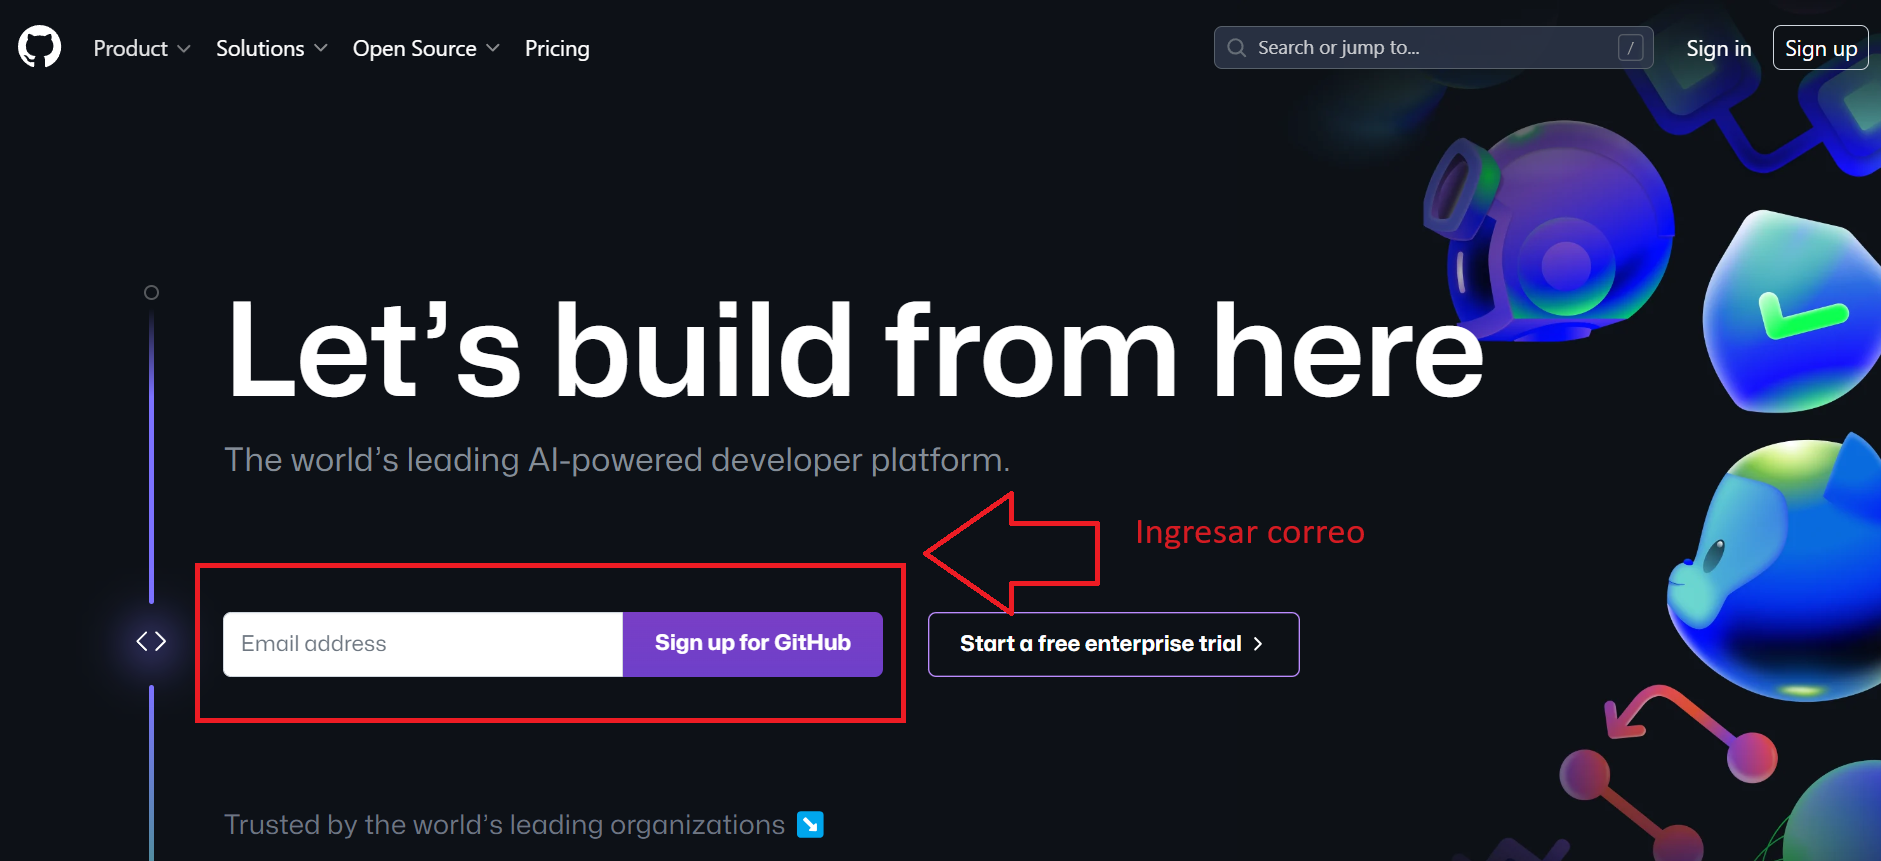
\includegraphics{images/github1.png}

La personalización de la cuenta se puede saltar haciendo click en
\textbf{skip} abajo de la selección de opciones

\begin{enumerate}
\def\labelenumi{\arabic{enumi}.}
\setcounter{enumi}{1}
\tightlist
\item
  Descargar e instalar Github Desktop
\end{enumerate}

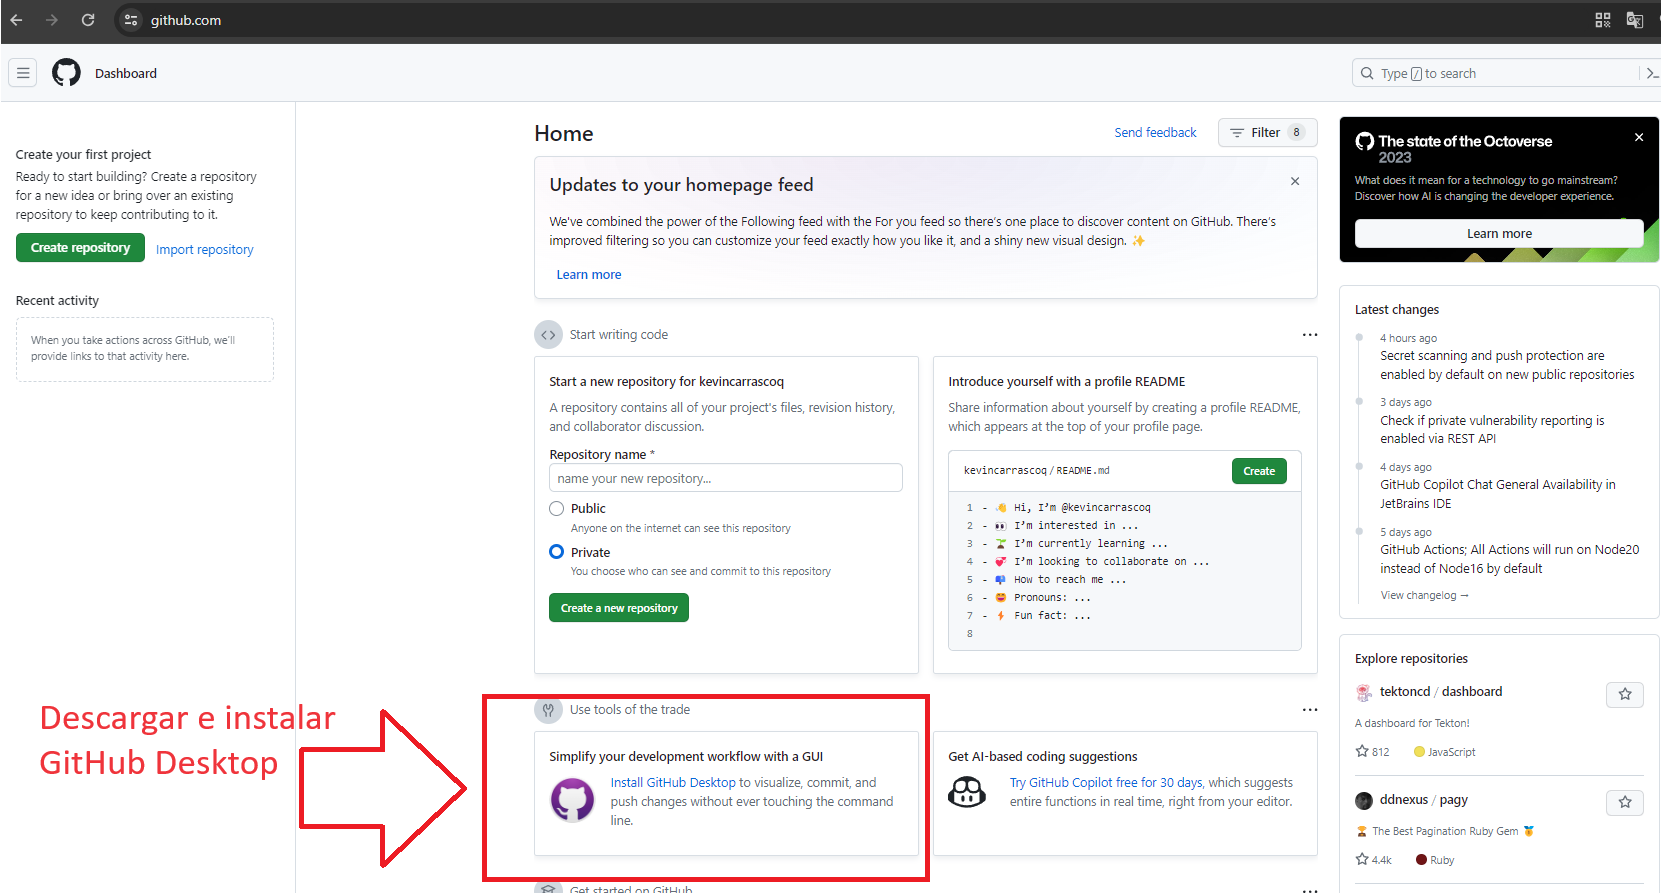
\includegraphics{images/github2.png}

\subsection{Crear repositorio}\label{crear-repositorio}

En la página principal de \href{https://github.com/}{github} hacer click
en el ícono de usuario de la esquina superior derecha y luego ir a Tus
repositorios

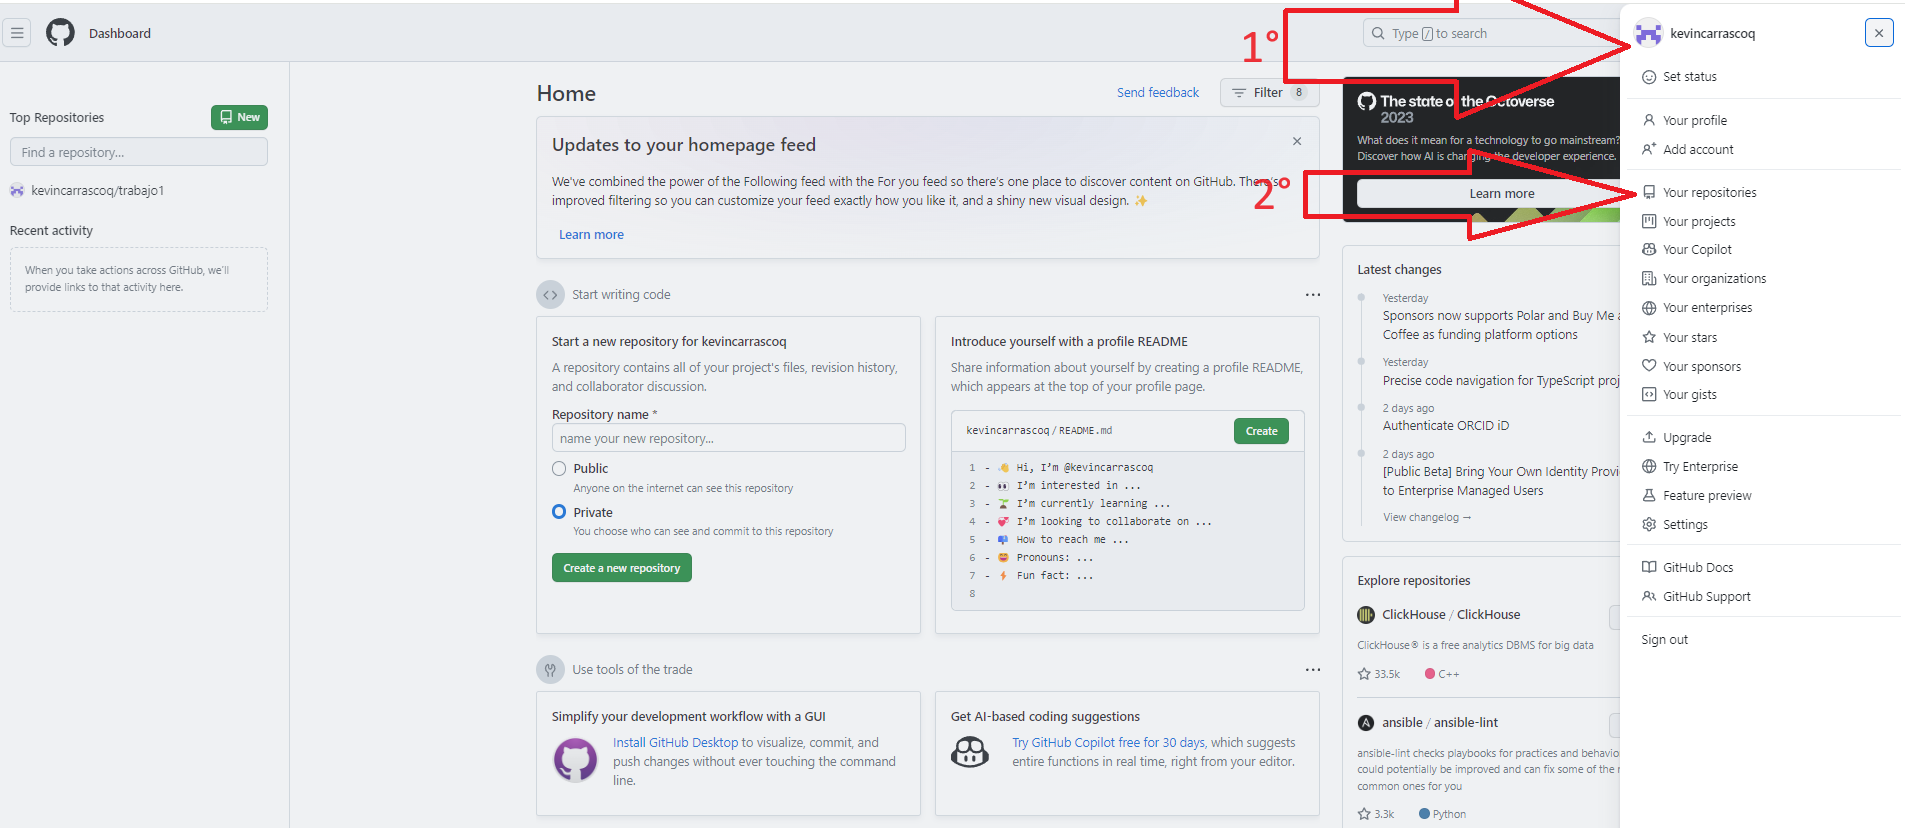
\includegraphics{images/repos.png}

Una vez accedemos a Tus repositorios hacemos click en New/Nuevo

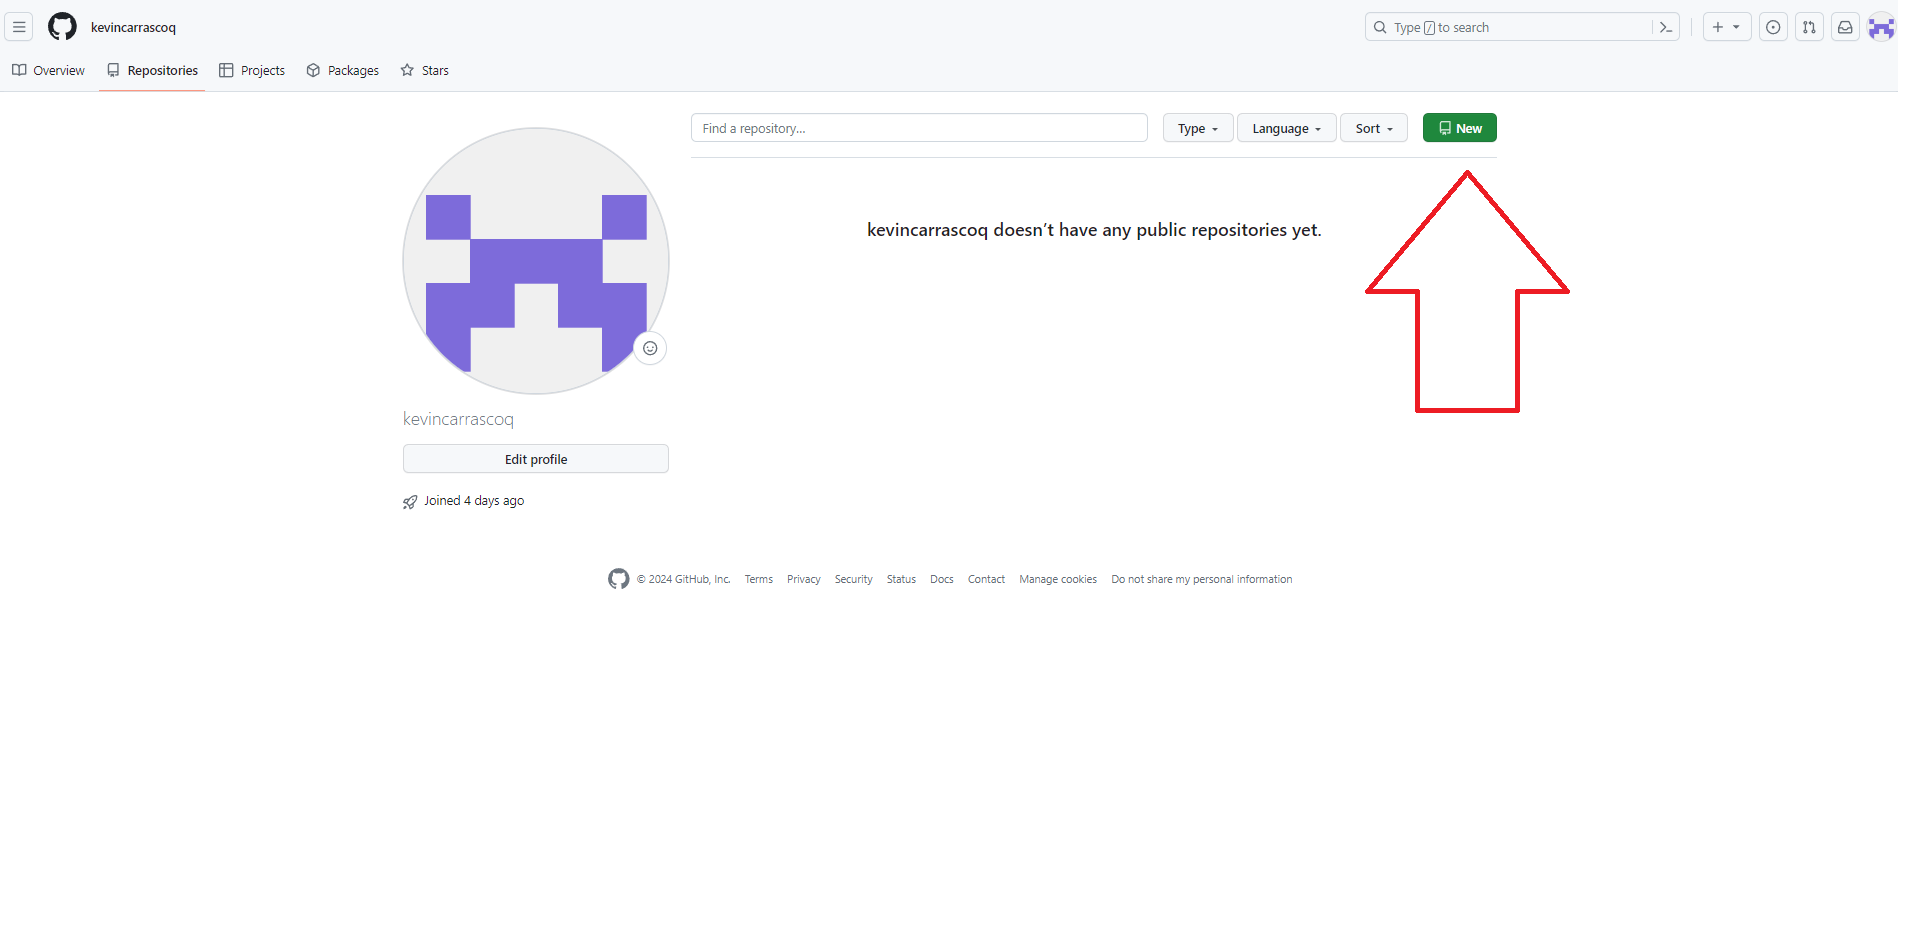
\includegraphics{images/repos2.png}

Luego le ponemos un nombre a nuestro repositorio, evitando siempre
espacios, ñ y tíldes, y apretamos Crear repositorio

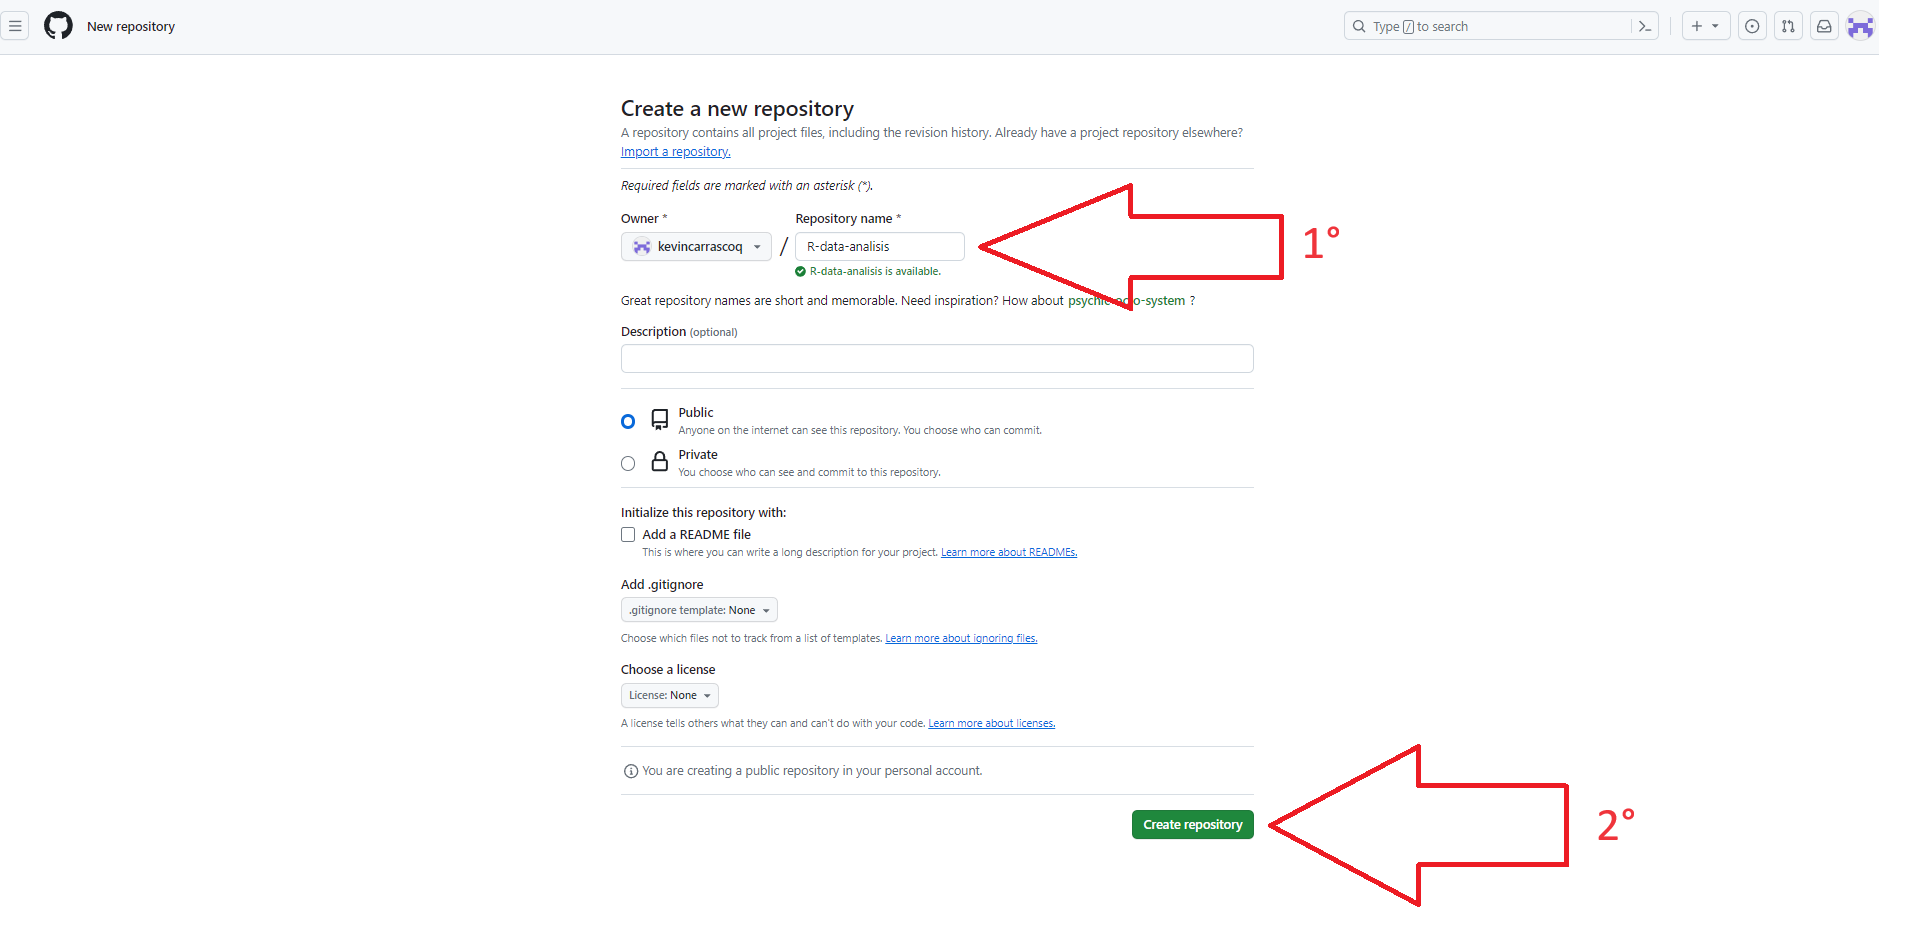
\includegraphics{images/repos3.png}

\begin{tcolorbox}[enhanced jigsaw, opacitybacktitle=0.6, colframe=quarto-callout-note-color-frame, breakable, toprule=.15mm, bottomrule=.15mm, toptitle=1mm, colback=white, bottomtitle=1mm, rightrule=.15mm, title=\textcolor{quarto-callout-note-color}{\faInfo}\hspace{0.5em}{Note}, leftrule=.75mm, coltitle=black, opacityback=0, titlerule=0mm, arc=.35mm, left=2mm, colbacktitle=quarto-callout-note-color!10!white]

Un buen nombre debería intentar resumir las principales características
del proyecto de investigación en no más de 3 o 4 conceptos (por ejemplo,
movilidad-social-AL para proyecto sobre movilidad social en América
Latina)

En esta oportunidad, una recomendación sería generar un repositorio
``ejercicios-practicos-RAD'' para almacenar los distintos scripts de
ejercicios prácticos que realizaremos en el curso R para el Análisis de
Datos.

Luego pueden generar un segundo repositorio que sea ``Trabajo RAD'' para
almacenar el desarrollo de sus trabajos de investigación.

\end{tcolorbox}

\subsection{Github desktop}\label{github-desktop}

Una vez creado un repositorio, lo que nos interesa es descargarlo. Al
abrir la aplicación de Github desktop por primera vez (descargada
anteriormente), nos debería aparecer la opción de clonar nuestro
repositorio R-data-analisis en la pantalla de inicio. Lo clonamos y
seleccionamos una carpeta de nuestro computador para almacenarlo.

Para todas las siguientes veces, las instrucciones son estas:

1- Apretamos Repositorio actual en la esquina superior izquierda

2- Apretamos añadir

3- Apretamos clonar repositorio\ldots{}

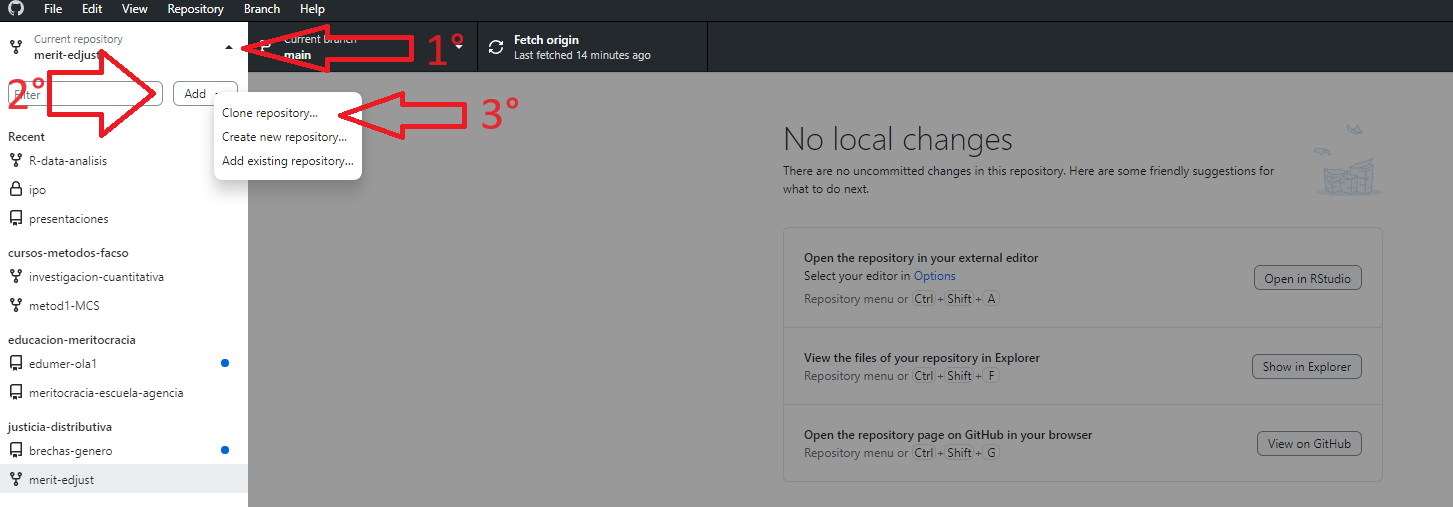
\includegraphics{images/clonar.png}

4- Seleccionamos nuestro repositorio

5- seleccionamos la carpeta donde se almacenará. Siempre evitando tener
tíldes, ñ y espacios en la dirección de almacenamiento y apretamos
`clone'.

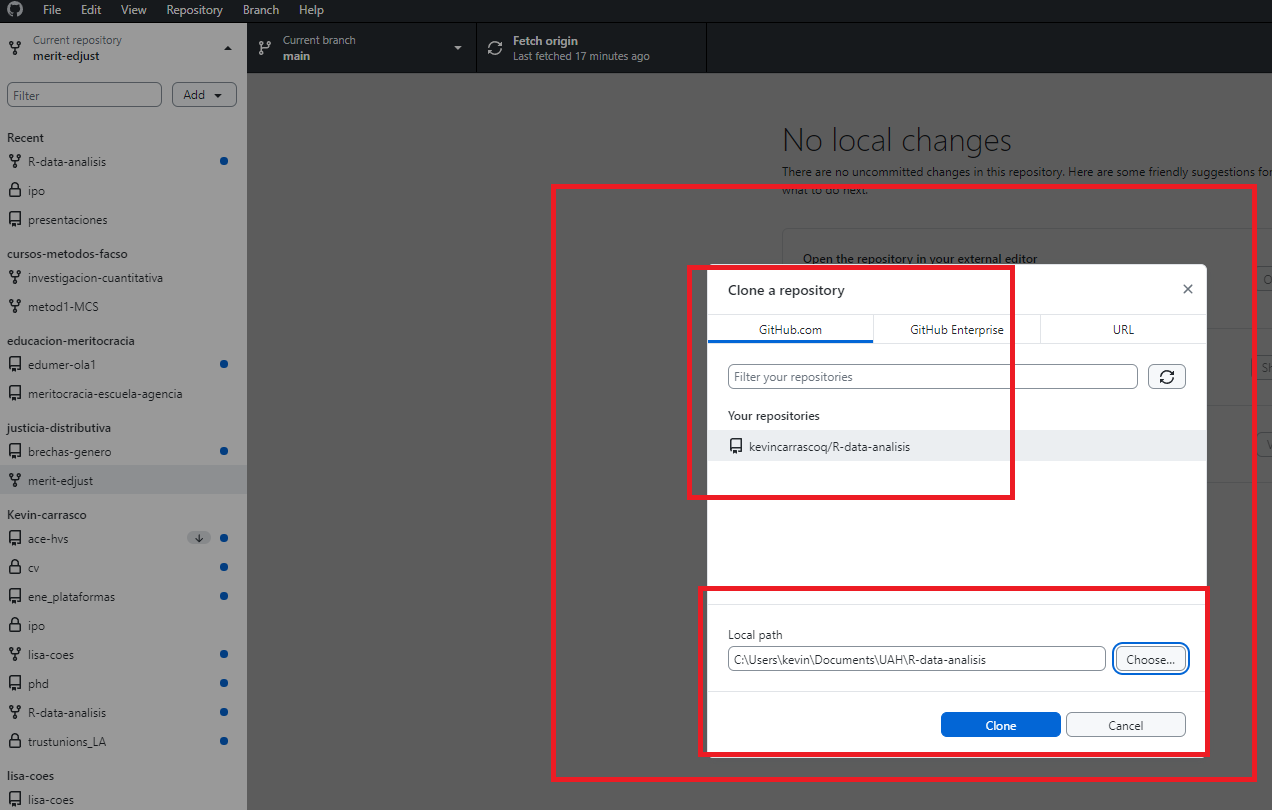
\includegraphics{images/clonar2.png}

\begin{tcolorbox}[enhanced jigsaw, opacitybacktitle=0.6, colframe=quarto-callout-note-color-frame, breakable, toprule=.15mm, bottomrule=.15mm, toptitle=1mm, colback=white, bottomtitle=1mm, rightrule=.15mm, title=\textcolor{quarto-callout-note-color}{\faInfo}\hspace{0.5em}{Note}, leftrule=.75mm, coltitle=black, opacityback=0, titlerule=0mm, arc=.35mm, left=2mm, colbacktitle=quarto-callout-note-color!10!white]

La aplicación de escritorio de Github es un poco más intuitiva y fácil
de usar. Sin embargo, RStudio también tiene una extensión para utilizar
github de manera directa dentro de la plataforma.

Mientras tanto utilicen Github Desktop en sus computadores personales.
Las siguientes clases en el laboratorio de computación de la UAH
utilizaremos Rstudio para clonar sus repositorios y hacer las
modificaciones correspondientes.

\end{tcolorbox}

7- Creamos las carpetas pertenecientes al protocolo IPO
(input-procesamiento-output) para organizar nuestro proyecto)

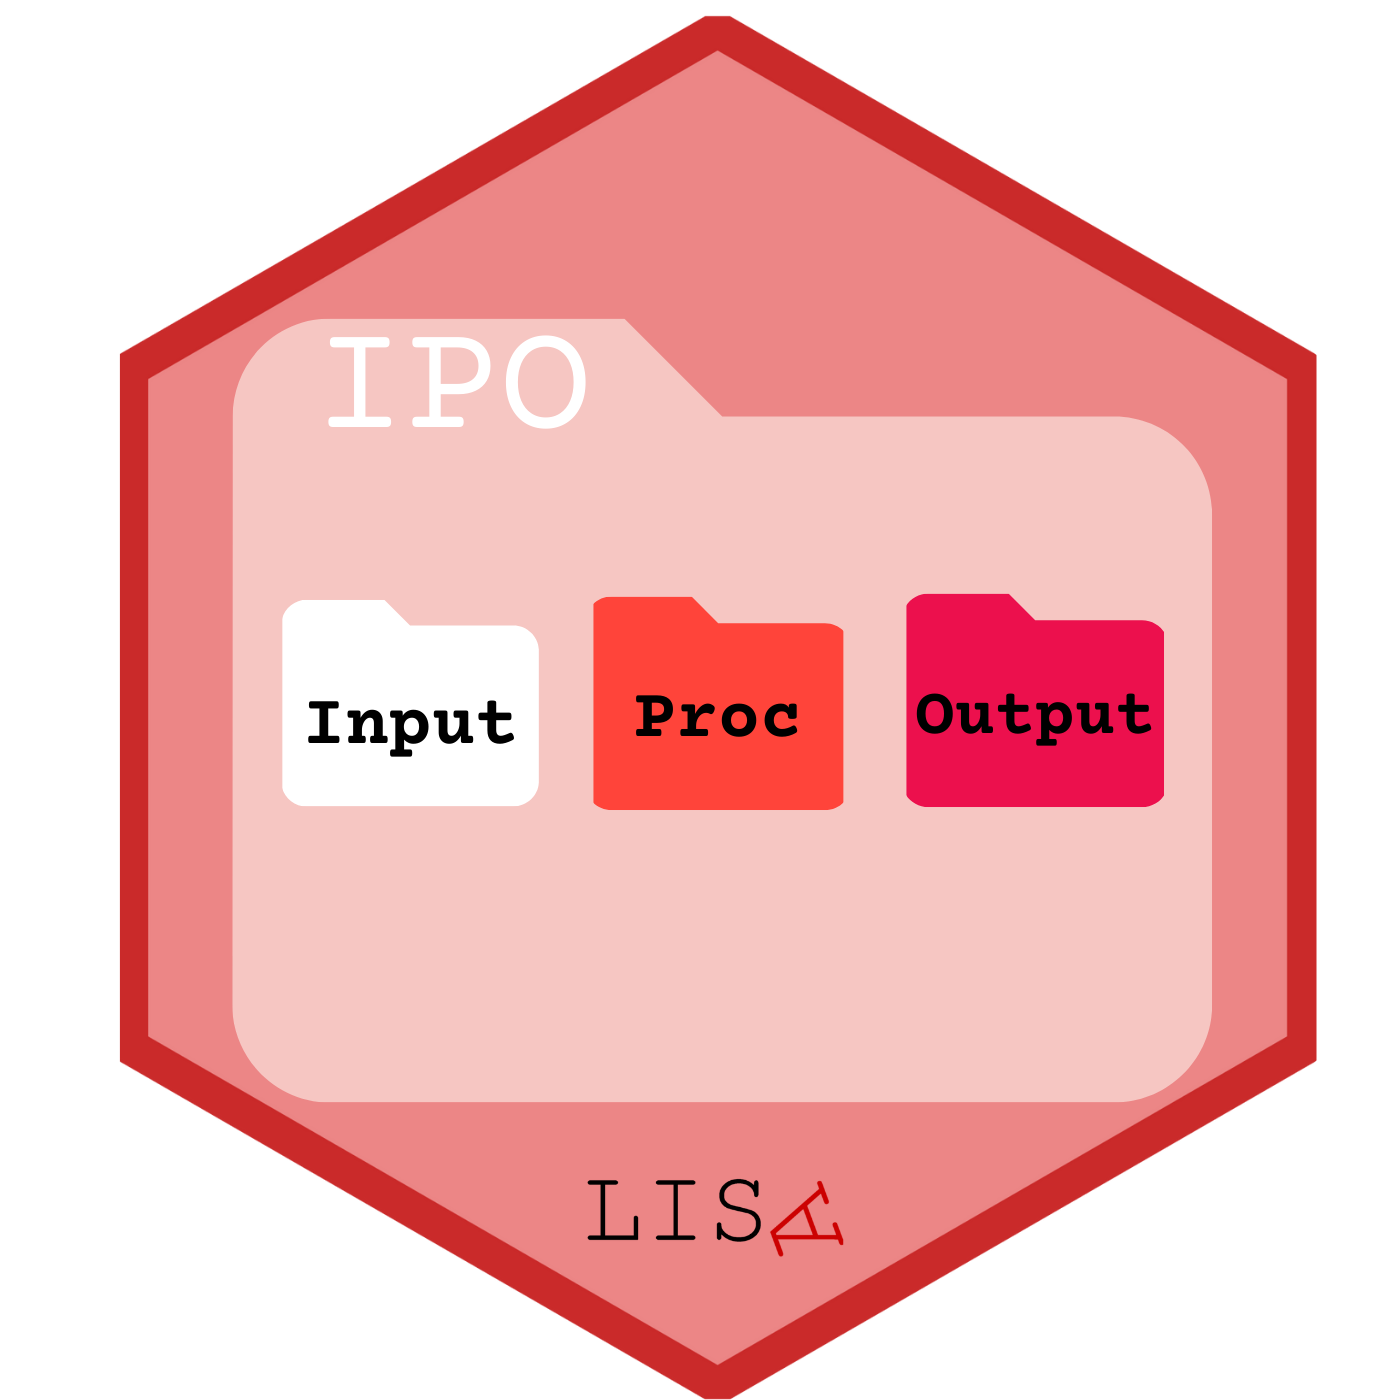
\includegraphics{images/ipo-hex.png}

\subsection{RStudio Projects}\label{rstudio-projects}

\begin{itemize}
\tightlist
\item
  File -\textgreater{} New Project
\end{itemize}

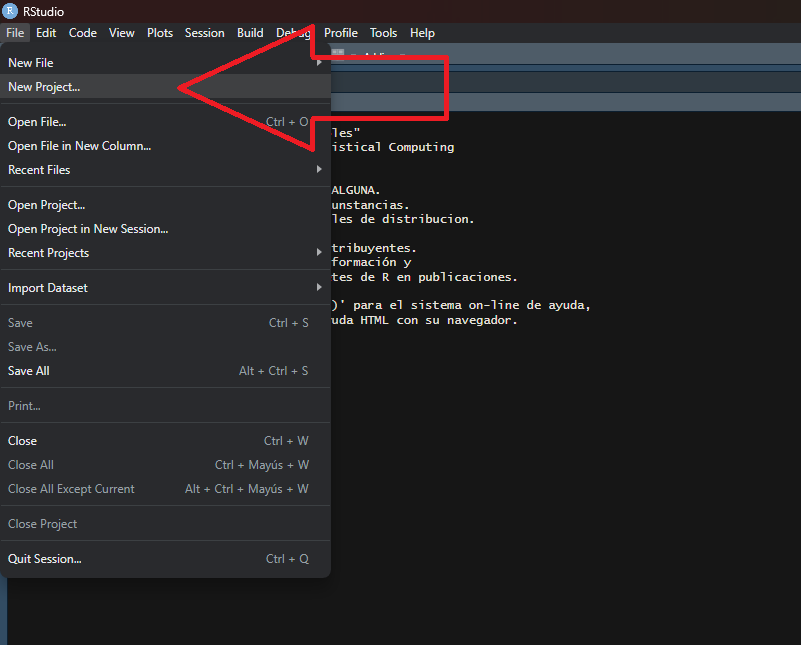
\includegraphics{images/project.png}

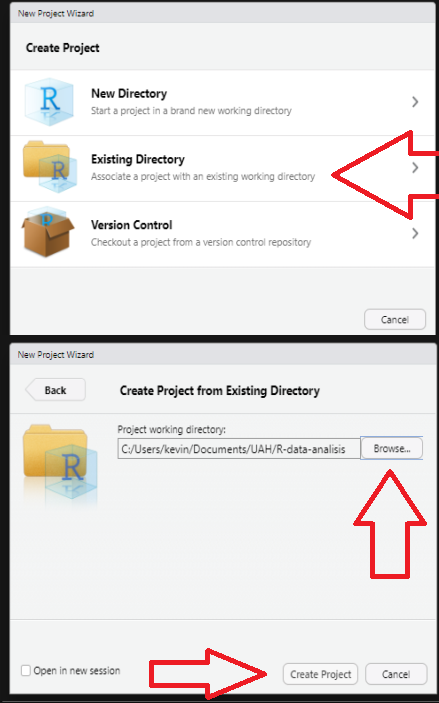
\includegraphics{images/project2.png}

\subsection{Abriendo la sesión de RStudio como
proyecto}\label{abriendo-la-sesiuxf3n-de-rstudio-como-proyecto}

\begin{itemize}
\item
  identificar en la carpeta respectiva el archivo .Rproj
\item
  ejecutar y se abre R / RStudio con ese directorio como raíz
\end{itemize}

\subsection{Rutas relativas en
código}\label{rutas-relativas-en-cuxf3digo}

\begin{itemize}
\item
  forma de ``señalar el camino'' para abrir y guardar archivos al
  interior de una carpeta de proyecto autocontenido (= sin referencias
  locales)
\item
  este camino tiene básicamente 3 direcciones:

  \begin{itemize}
  \item
    bajar -\textgreater{} hacia subcarpetas
  \item
    subir -\textgreater{} hacia carpetas superiores
  \item
    subir y bajar -\textgreater{} hacia otras subcarpetas
  \end{itemize}
\end{itemize}

\subsubsection{bajando}\label{bajando}

\begin{itemize}
\item
  para \textbf{``bajar''} hacia a una subcarpeta, simplemente damos la
  ruta de la carpeta/archivo

  \begin{itemize}
  \item
    ej: si estoy en el archivo paper.Rmd (directorio raíz), y quiero
    incluir una imagen (directorio input/images/imagen.jpg), entonces la
    ruta es \texttt{input/images/imagen.jpg}
  \item
    o para señalar la ruta al bib desde paper.Rmd (en raíz):
    \texttt{input/bib/referencias.bib}
  \end{itemize}
\end{itemize}

\subsubsection{subiendo}\label{subiendo}

\begin{itemize}
\item
  para \textbf{subir} se utilizan los caracteres \texttt{../} por cada
  nivel.
\item
  Ej: si quiero guardar una tabla en el directorio raíz generada desde
  un archivo de código en la subcarpeta proc, entonces la ruta es
  \texttt{../tabla.html}
\end{itemize}

\subsubsection{subiendo y bajando}\label{subiendo-y-bajando}

\begin{itemize}
\item
  combinación de las anteriores
\item
  Ej: para abrir la base de datos original en la subcarpeta input/data
  desde el código de procesamiento en la subcarpeta proc, entonces:
\end{itemize}

\texttt{../input/data/original.dat}

\section{Quarto}\label{quarto}

La escritura en Quarto tiene algunos códigos o funciones, aquí un
resumen de su mayoría:

\begin{longtable}[]{@{}
  >{\raggedright\arraybackslash}p{(\columnwidth - 2\tabcolsep) * \real{0.5000}}
  >{\raggedright\arraybackslash}p{(\columnwidth - 2\tabcolsep) * \real{0.5000}}@{}}
\toprule\noalign{}
\begin{minipage}[b]{\linewidth}\raggedright
Código
\end{minipage} & \begin{minipage}[b]{\linewidth}\raggedright
Así se ve
\end{minipage} \\
\midrule\noalign{}
\endhead
\bottomrule\noalign{}
\endlastfoot
\begin{minipage}[t]{\linewidth}\raggedright
\begin{verbatim}
Algo de texto en el párrafo.

Más texto
espacio entre lineas.
\end{verbatim}
\end{minipage} & Algo de texto.

Algo de texto en el párrafo. Siempre utilizando espacios para dividir
párrafos \\
\texttt{*Cursivas*} & \emph{Cursivas} \\
\texttt{**Negrita**} & \textbf{Negrita} \\
\texttt{\#\ Título\ 1} & \begin{minipage}[t]{\linewidth}\raggedright
\section{Título 1}\label{tuxedtulo-1}
\end{minipage} \\
\texttt{\#\#\ Título\ 2} & \begin{minipage}[t]{\linewidth}\raggedright
\subsection{Título 2}\label{tuxedtulo-2}
\end{minipage} \\
\texttt{\#\#\#\ Título\ 3} & \begin{minipage}[t]{\linewidth}\raggedright
\subsubsection{Título 3}\label{tuxedtulo-3}
\end{minipage} \\
(puedes llegar hasta un título N° 6 con \texttt{\#\#\#\#\#\#}) & \\
\texttt{{[}Texto\ enlace{]}(https://quarto.org/)} &
\href{https://quarto.org/}{Texto enlace} \\
\texttt{!{[}Texto\ imagen{]}(/path/to/image.png)} &
\begin{minipage}[t]{\linewidth}\raggedright
\begin{figure}[H]

{\centering 
\includegraphics{images/lisa_icon.png}

}

\caption{Texto imagen}

\end{figure}%
\end{minipage} \\
\texttt{\textgreater{}\ Citas} &
\begin{minipage}[t]{\linewidth}\raggedright
\begin{quote}
Citas
\end{quote}
\end{minipage} \\
\begin{minipage}[t]{\linewidth}\raggedright
\begin{verbatim}
1. Una
2. lista
3 ordenada
\end{verbatim}
\end{minipage} & \begin{minipage}[t]{\linewidth}\raggedright
\begin{enumerate}
\def\labelenumi{\arabic{enumi}.}
\item
  Una
\item
  lista
\item
  ordenada
\end{enumerate}
\end{minipage} \\
\begin{minipage}[t]{\linewidth}\raggedright
\begin{verbatim}
- Otro
- tipo
- de lista
\end{verbatim}
\end{minipage} & \begin{minipage}[t]{\linewidth}\raggedright
\begin{itemize}
\item
  Otro
\item
  tipo
\item
  de lista
\end{itemize}
\end{minipage} \\
\end{longtable}

\begin{enumerate}
\def\labelenumi{\arabic{enumi}.}
\tightlist
\item
  Abrimos nuestro Rproject y creamos un nuevo documento de Quarto file
  --\textgreater{} new file --\textgreater{} Quarto document
\end{enumerate}

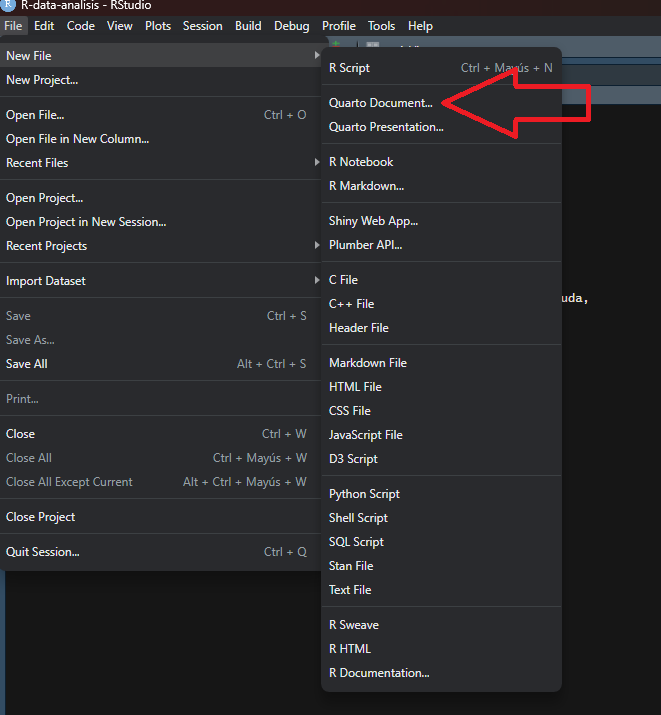
\includegraphics{images/quarto-2.png}

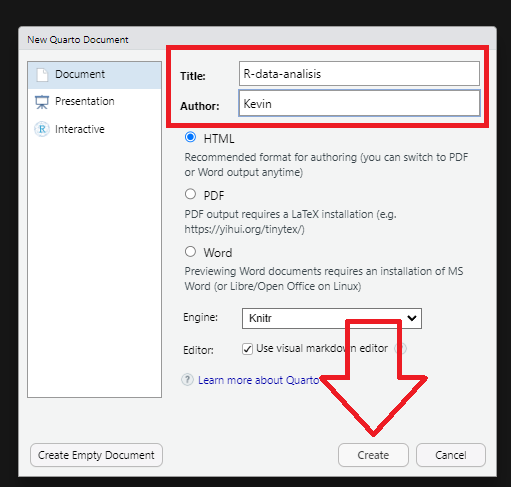
\includegraphics{images/quarto2-2.png}

\begin{tcolorbox}[enhanced jigsaw, opacitybacktitle=0.6, colframe=quarto-callout-note-color-frame, breakable, toprule=.15mm, bottomrule=.15mm, toptitle=1mm, colback=white, bottomtitle=1mm, rightrule=.15mm, title=\textcolor{quarto-callout-note-color}{\faInfo}\hspace{0.5em}{Note}, leftrule=.75mm, coltitle=black, opacityback=0, titlerule=0mm, arc=.35mm, left=2mm, colbacktitle=quarto-callout-note-color!10!white]

YAML: Lenguaje de programación. Es un formato de serialización de datos
que proporcionan un mecanismo de intercambio de datos legible por
humanos. Dan formato a los datos de manera estandarizada para su
intercambio entre aplicaciones de software.

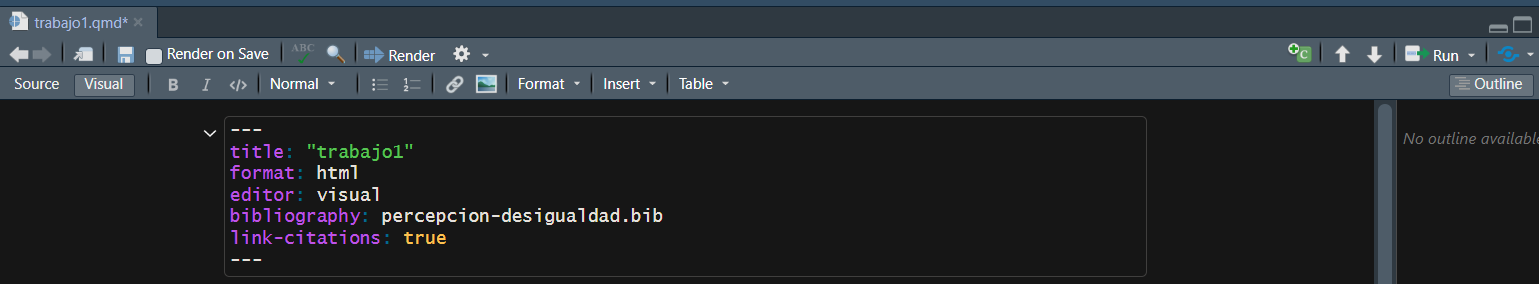
\includegraphics{images/yaml.png}

\end{tcolorbox}

\begin{verbatim}
---
title: "Mi Documento"
format:
  html:
    toc: true
    number-sections: true
---
\end{verbatim}

Luego, podemos escribir en el documento, separando por títulos (\#) cada
sección. La jerarquía de los títulos se establece según la cantidad de
`\#'.

A continuación, en esta guía combinaremos el paso-a-paso de crear un
documento dinámico con quarto, a la vez que vamos viendo distintas
funciones de este proceso.

Por ejemplo, como hacer una nota al pie\footnote{Esta es la nota al pie}.
Para hacerlo, solo debemos escribir {[} \^{}2{]} pero sin el espacio
entre los corchetes. Luego, en otra línea escribimos {[}\^{}2{]}: Esta
es la nota al pie

\section{Código de análisis de
ejemplo}\label{cuxf3digo-de-anuxe1lisis-de-ejemplo}

Para poder escribir código de análisis en un documento Quarto debemos
generar trozo de código llamado `Chunk', que se puede crear con
ctrl+alt+i o directamente en el menú de arriba en `Code -\textgreater{}
Insert Chunk'.

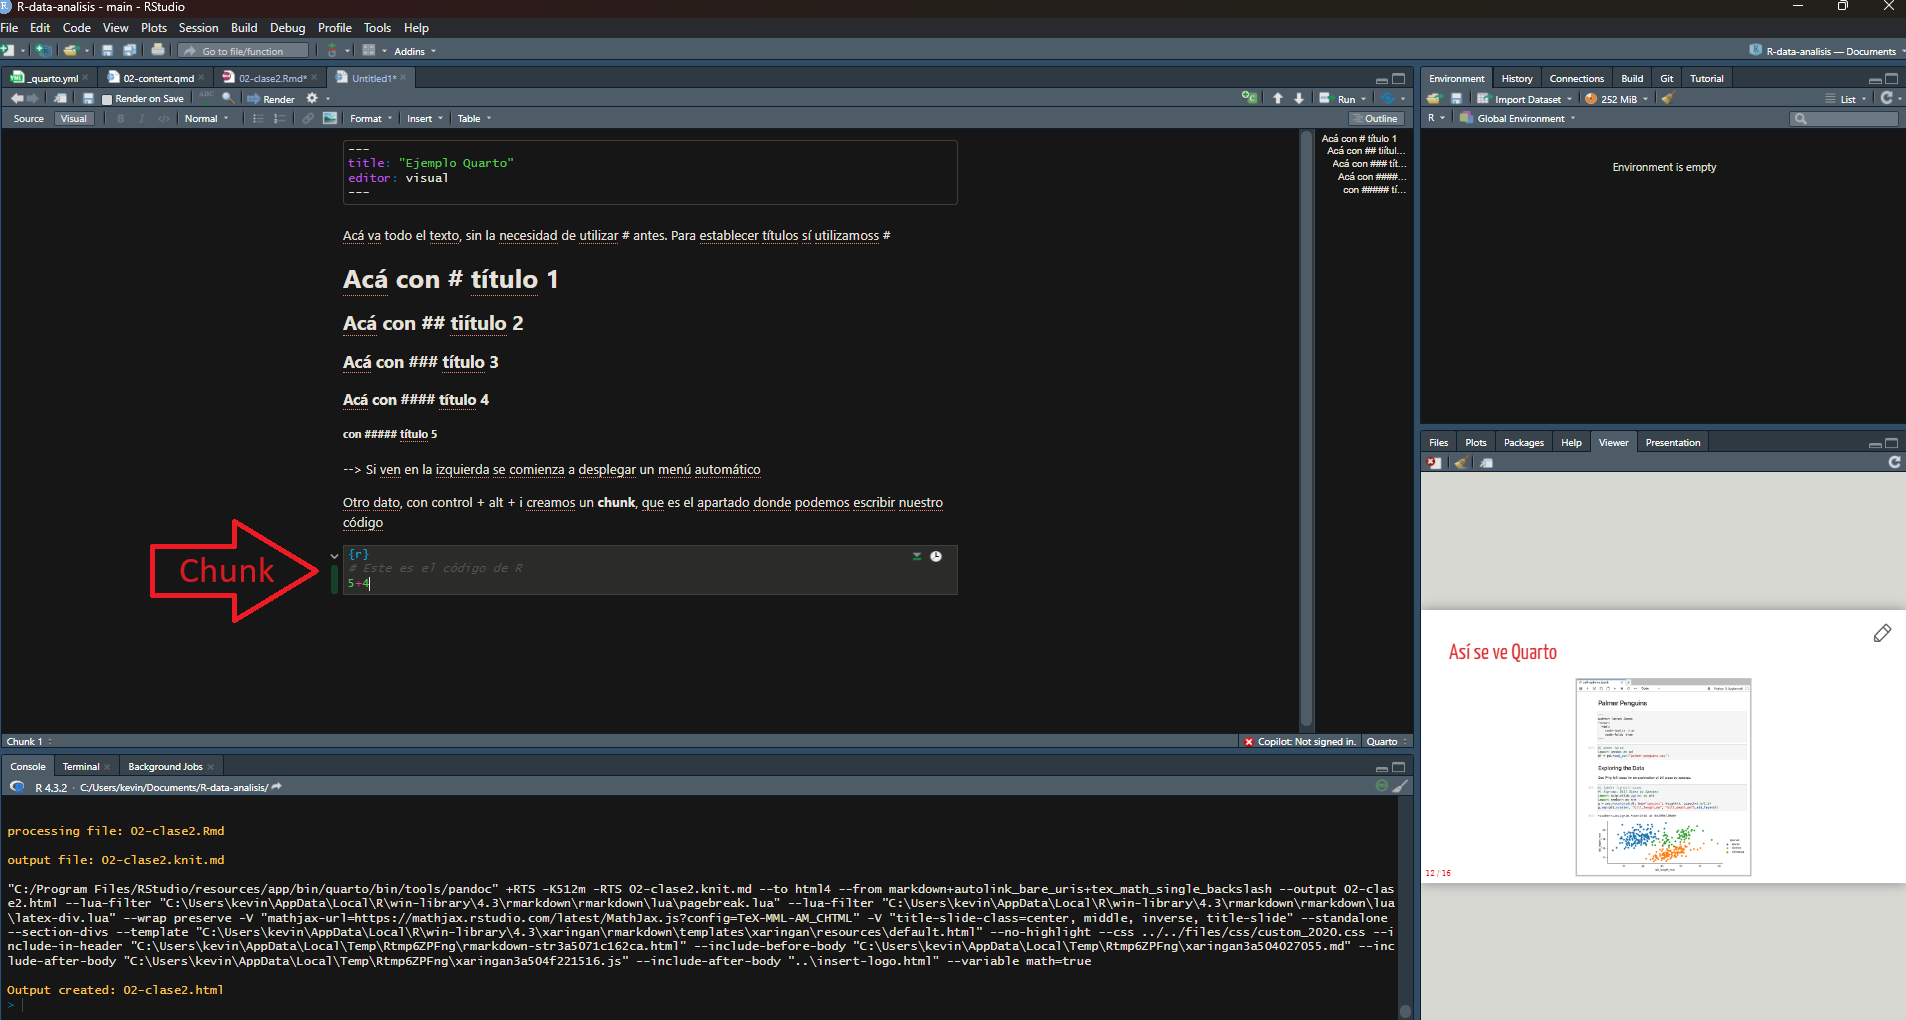
\includegraphics{images/quarto3.png}

\subsection{Cargar paquetes}\label{cargar-paquetes}

\begin{Shaded}
\begin{Highlighting}[]
\NormalTok{pacman}\SpecialCharTok{::}\FunctionTok{p\_load}\NormalTok{(sjlabelled,}
\NormalTok{               dplyr, }\CommentTok{\#Manipulacion de datos}
\NormalTok{              stargazer, }\CommentTok{\#Tablas}
\NormalTok{              sjmisc, }\CommentTok{\# Tablas}
\NormalTok{              summarytools, }\CommentTok{\# Tablas}
\NormalTok{              kableExtra, }\CommentTok{\#Tablas}
\NormalTok{              sjPlot, }\CommentTok{\#Tablas y gráficos}
\NormalTok{              corrplot, }\CommentTok{\# Correlaciones}
\NormalTok{              sessioninfo, }\CommentTok{\# Información de la sesión de trabajo}
\NormalTok{              ggplot2) }\CommentTok{\# Para la mayoría de los gráficos}
\end{Highlighting}
\end{Shaded}

\subsection{Cargar bases de datos}\label{cargar-bases-de-datos}

Cargamos ambas bases de datos desde internet

\begin{Shaded}
\begin{Highlighting}[]
\FunctionTok{load}\NormalTok{(}\FunctionTok{url}\NormalTok{(}\StringTok{"https://github.com/Kevin{-}carrasco/R{-}data{-}analisis/raw/main/files/data/latinobarometro\_total.RData"}\NormalTok{)) }\CommentTok{\#Cargar base de datos}
\FunctionTok{load}\NormalTok{(}\FunctionTok{url}\NormalTok{(}\StringTok{"https://github.com/Kevin{-}carrasco/R{-}data{-}analisis/raw/main/files/data/data\_wvs.RData"}\NormalTok{)) }\CommentTok{\#Cargar base de datos}
\end{Highlighting}
\end{Shaded}

Para trabajar con ambas bases, agruparemos las variables de interés por
país, por lo que ya no trabajaremos directamente con individuos.

\begin{Shaded}
\begin{Highlighting}[]
\NormalTok{context\_data }\OtherTok{\textless{}{-}}\NormalTok{ wvs }\SpecialCharTok{\%\textgreater{}\%} \FunctionTok{group\_by}\NormalTok{(B\_COUNTRY) }\SpecialCharTok{\%\textgreater{}\%} \CommentTok{\# Agrupar por país}
  \FunctionTok{summarise}\NormalTok{(}\AttributeTok{gdp =} \FunctionTok{mean}\NormalTok{(GDPpercap1, }\AttributeTok{na.rm =} \ConstantTok{TRUE}\NormalTok{), }\CommentTok{\# Promedio de GDP per capita}
         \AttributeTok{life\_exp =} \FunctionTok{mean}\NormalTok{(lifeexpect, }\AttributeTok{na.rm =} \ConstantTok{TRUE}\NormalTok{), }\CommentTok{\# Promedio esperanza de vida}
         \AttributeTok{gini =} \FunctionTok{mean}\NormalTok{(giniWB, }\AttributeTok{na.rm =} \ConstantTok{TRUE}\NormalTok{)) }\SpecialCharTok{\%\textgreater{}\%}  \CommentTok{\# Promedio gini}
  \FunctionTok{rename}\NormalTok{(}\AttributeTok{idenpa=}\NormalTok{B\_COUNTRY) }\CommentTok{\# Para poder vincular ambas bases, es necesario que la variable de identificación se llamen igual}
\NormalTok{context\_data}\SpecialCharTok{$}\NormalTok{idenpa }\OtherTok{\textless{}{-}} \FunctionTok{as.numeric}\NormalTok{(context\_data}\SpecialCharTok{$}\NormalTok{idenpa) }\CommentTok{\# Como era categórica, la dejamos numérica}

\NormalTok{proc\_data }\OtherTok{\textless{}{-}}\NormalTok{ proc\_data }\SpecialCharTok{\%\textgreater{}\%} \FunctionTok{group\_by}\NormalTok{(idenpa) }\SpecialCharTok{\%\textgreater{}\%}  \CommentTok{\# agrupamos por país}
  \FunctionTok{summarise}\NormalTok{(}\AttributeTok{promedio =} \FunctionTok{mean}\NormalTok{(conf\_inst, }\AttributeTok{na.rm =} \ConstantTok{TRUE}\NormalTok{)) }\CommentTok{\# promedio de confianza en instituciones por país}
\end{Highlighting}
\end{Shaded}

\subsection{Unir bases de datos}\label{unir-bases-de-datos}

Para vincular nuestras bases de datos existen múltiples opciones, la
primera es `merge' de R base y las siguientes tres vienen desde dplyr:
`right\_join', `full\_join' y `left\_join'. Cada una tiene sus propias
potencialidades y limitaciones y dependerá de cada caso cuál usemos

\subsubsection{Probemos merge}\label{probemos-merge}

\begin{Shaded}
\begin{Highlighting}[]
\NormalTok{data }\OtherTok{\textless{}{-}} \FunctionTok{merge}\NormalTok{(proc\_data, context\_data, }\AttributeTok{by=}\StringTok{"idenpa"}\NormalTok{)}
\end{Highlighting}
\end{Shaded}

\begin{Shaded}
\begin{Highlighting}[]
\NormalTok{data }\OtherTok{\textless{}{-}}\NormalTok{ data }\SpecialCharTok{\%\textgreater{}\%}
  \FunctionTok{mutate}\NormalTok{(}\AttributeTok{idenpa =} \FunctionTok{as.character}\NormalTok{(idenpa)) }\SpecialCharTok{\%\textgreater{}\%}
  \FunctionTok{mutate}\NormalTok{(}\AttributeTok{idenpa =} \FunctionTok{case\_when}\NormalTok{(}
\NormalTok{    idenpa }\SpecialCharTok{==} \StringTok{"32"} \SpecialCharTok{\textasciitilde{}} \StringTok{"Argentina"}\NormalTok{,}
\NormalTok{    idenpa }\SpecialCharTok{==} \StringTok{"68"} \SpecialCharTok{\textasciitilde{}} \StringTok{"Bolivia"}\NormalTok{,}
\NormalTok{    idenpa }\SpecialCharTok{==} \StringTok{"76"} \SpecialCharTok{\textasciitilde{}} \StringTok{"Brasil"}\NormalTok{,}
\NormalTok{    idenpa }\SpecialCharTok{==} \StringTok{"152"} \SpecialCharTok{\textasciitilde{}} \StringTok{"Chile"}\NormalTok{,}
\NormalTok{    idenpa }\SpecialCharTok{==} \StringTok{"170"} \SpecialCharTok{\textasciitilde{}} \StringTok{"Colombia"}\NormalTok{,}
\NormalTok{    idenpa }\SpecialCharTok{==} \StringTok{"188"} \SpecialCharTok{\textasciitilde{}} \StringTok{"Costa Rica"}\NormalTok{,}
\NormalTok{    idenpa }\SpecialCharTok{==} \StringTok{"214"} \SpecialCharTok{\textasciitilde{}} \StringTok{"Cuba"}\NormalTok{,}
\NormalTok{    idenpa }\SpecialCharTok{==} \StringTok{"218"} \SpecialCharTok{\textasciitilde{}} \StringTok{"República Dominicana"}\NormalTok{,}
\NormalTok{    idenpa }\SpecialCharTok{==} \StringTok{"222"} \SpecialCharTok{\textasciitilde{}} \StringTok{"Ecuador"}\NormalTok{,}
\NormalTok{    idenpa }\SpecialCharTok{==} \StringTok{"320"} \SpecialCharTok{\textasciitilde{}} \StringTok{"El Salvador"}\NormalTok{,}
\NormalTok{    idenpa }\SpecialCharTok{==} \StringTok{"340"} \SpecialCharTok{\textasciitilde{}} \StringTok{"Guatemala"}\NormalTok{,}
\NormalTok{    idenpa }\SpecialCharTok{==} \StringTok{"484"} \SpecialCharTok{\textasciitilde{}} \StringTok{"Honduras"}\NormalTok{,}
\NormalTok{    idenpa }\SpecialCharTok{==} \StringTok{"558"} \SpecialCharTok{\textasciitilde{}} \StringTok{"México"}\NormalTok{,}
\NormalTok{    idenpa }\SpecialCharTok{==} \StringTok{"591"} \SpecialCharTok{\textasciitilde{}} \StringTok{"Nicaragua"}\NormalTok{,}
\NormalTok{    idenpa }\SpecialCharTok{==} \StringTok{"600"} \SpecialCharTok{\textasciitilde{}} \StringTok{"Panamá"}\NormalTok{,}
\NormalTok{    idenpa }\SpecialCharTok{==} \StringTok{"604"} \SpecialCharTok{\textasciitilde{}} \StringTok{"Paraguay"}\NormalTok{,}
\NormalTok{    idenpa }\SpecialCharTok{==} \StringTok{"858"} \SpecialCharTok{\textasciitilde{}} \StringTok{"Uruguay"}\NormalTok{,}
\NormalTok{    idenpa }\SpecialCharTok{==} \StringTok{"862"} \SpecialCharTok{\textasciitilde{}} \StringTok{"Venezuela"}\NormalTok{))}

\NormalTok{data}\SpecialCharTok{$}\NormalTok{gdp }\OtherTok{\textless{}{-}} \FunctionTok{as.numeric}\NormalTok{(data}\SpecialCharTok{$}\NormalTok{gdp)}
\NormalTok{data}\SpecialCharTok{$}\NormalTok{gdp[data}\SpecialCharTok{$}\NormalTok{gdp}\SpecialCharTok{==}\DecValTok{0}\NormalTok{] }\OtherTok{\textless{}{-}} \ConstantTok{NA}
\NormalTok{data }\OtherTok{\textless{}{-}} \FunctionTok{na.omit}\NormalTok{(data)}
\end{Highlighting}
\end{Shaded}

\subsubsection{Guardamos esta nueva base en nuestra carpeta
input}\label{guardamos-esta-nueva-base-en-nuestra-carpeta-input}

\begin{Shaded}
\begin{Highlighting}[]
\FunctionTok{save}\NormalTok{(data, }\AttributeTok{file=}\StringTok{"input/data/proc/data.RData"}\NormalTok{)}
\end{Highlighting}
\end{Shaded}

\subsection{Visualizaciones}\label{visualizaciones}

Podemos establecer referencias cruzadas para las tablas y gráficos
dentro del texto, para poder automatizarlo, como ejemplo así, pero
dentro del chunk:

\#\textbar{} label: tbl-sjmisc

\#\textbar{} tbl-cap: ``Descriptivos con sjmisc''

\subsubsection{Descriptivos}\label{descriptivos}

El Chunk se debería ver así:

\#\textbar{} label: tbl-sjmisc

\#\textbar{} tbl-cap: ``Descriptivos con sjmisc''

sjmisc::descr(data,

\begin{verbatim}
  show = c("label","range", "mean", "sd", "NA.prc", "n"))%>% # Selecciona estadísticos

  kable(.,"markdown") # Esto es para que se vea bien en quarto
\end{verbatim}

\begin{Shaded}
\begin{Highlighting}[]
\NormalTok{sjmisc}\SpecialCharTok{::}\FunctionTok{descr}\NormalTok{(data,}
      \AttributeTok{show =} \FunctionTok{c}\NormalTok{(}\StringTok{"label"}\NormalTok{,}\StringTok{"range"}\NormalTok{, }\StringTok{"mean"}\NormalTok{, }\StringTok{"sd"}\NormalTok{, }\StringTok{"NA.prc"}\NormalTok{, }\StringTok{"n"}\NormalTok{))}\SpecialCharTok{\%\textgreater{}\%} \CommentTok{\# Selecciona estadísticos}
      \FunctionTok{kable}\NormalTok{(.,}\StringTok{"markdown"}\NormalTok{) }\CommentTok{\# Esto es para que se vea bien en quarto}
\end{Highlighting}
\end{Shaded}

\begin{longtable}[]{@{}
  >{\raggedright\arraybackslash}p{(\columnwidth - 14\tabcolsep) * \real{0.0366}}
  >{\raggedright\arraybackslash}p{(\columnwidth - 14\tabcolsep) * \real{0.1098}}
  >{\raggedright\arraybackslash}p{(\columnwidth - 14\tabcolsep) * \real{0.1098}}
  >{\raggedleft\arraybackslash}p{(\columnwidth - 14\tabcolsep) * \real{0.0366}}
  >{\raggedleft\arraybackslash}p{(\columnwidth - 14\tabcolsep) * \real{0.0854}}
  >{\raggedleft\arraybackslash}p{(\columnwidth - 14\tabcolsep) * \real{0.1463}}
  >{\raggedleft\arraybackslash}p{(\columnwidth - 14\tabcolsep) * \real{0.1463}}
  >{\raggedright\arraybackslash}p{(\columnwidth - 14\tabcolsep) * \real{0.3293}}@{}}

\caption{\label{tbl-sjmisc}Descriptivos con sjmisc}

\tabularnewline

\toprule\noalign{}
\begin{minipage}[b]{\linewidth}\raggedright
\end{minipage} & \begin{minipage}[b]{\linewidth}\raggedright
var
\end{minipage} & \begin{minipage}[b]{\linewidth}\raggedright
label
\end{minipage} & \begin{minipage}[b]{\linewidth}\raggedleft
n
\end{minipage} & \begin{minipage}[b]{\linewidth}\raggedleft
NA.prc
\end{minipage} & \begin{minipage}[b]{\linewidth}\raggedleft
mean
\end{minipage} & \begin{minipage}[b]{\linewidth}\raggedleft
sd
\end{minipage} & \begin{minipage}[b]{\linewidth}\raggedright
range
\end{minipage} \\
\midrule\noalign{}
\endhead
\bottomrule\noalign{}
\endlastfoot
4 & promedio & promedio & 11 & 0 & 3.40077 & 1.016976 & 3.59
(2.3-5.9) \\
1 & gdp & gdp & 11 & 0 & 15528.18364 & 6480.045512 & 19523.79
(5631.2-25154.99) \\
3 & life\_exp & life\_exp & 11 & 0 & 75.90909 & 2.286593 & 8.8
(71.24-80.04) \\
2 & gini & gini & 11 & 0 & 45.46364 & 4.156266 & 14.2 (39.7-53.9) \\

\end{longtable}

Luego de establecer el link y el nombre de la tabla, podemos referenciar
acá con un @, así: @ tbl-sjmisc (pero junto), y que se vería así
Table~\ref{tbl-sjmisc}

\subsubsection{Gráficos}\label{gruxe1ficos}

Y para los gráficos se hace de la misma forma:

\#\textbar{} label: fig-gdp

\#\textbar{} fig-cap: ``Plots''

\begin{Shaded}
\begin{Highlighting}[]
\NormalTok{graph1}\OtherTok{\textless{}{-}}\FunctionTok{ggplot}\NormalTok{(data, }\FunctionTok{aes}\NormalTok{(}\AttributeTok{x =}\NormalTok{ idenpa, }\AttributeTok{y =}\NormalTok{ gdp)) }\SpecialCharTok{+}
  \FunctionTok{geom\_point}\NormalTok{() }\SpecialCharTok{+}
  \FunctionTok{labs}\NormalTok{(}\AttributeTok{x =} \StringTok{"País"}\NormalTok{, }\AttributeTok{y =} \StringTok{"Gdp"}\NormalTok{) }\SpecialCharTok{+}
  \FunctionTok{theme\_minimal}\NormalTok{()}\SpecialCharTok{+}
  \FunctionTok{theme}\NormalTok{(}\AttributeTok{axis.text.x =} \FunctionTok{element\_text}\NormalTok{(}\AttributeTok{angle =} \DecValTok{45}\NormalTok{, }\AttributeTok{hjust =} \DecValTok{1}\NormalTok{))}

\NormalTok{graph1}
\end{Highlighting}
\end{Shaded}

\begin{figure}[H]

\centering{

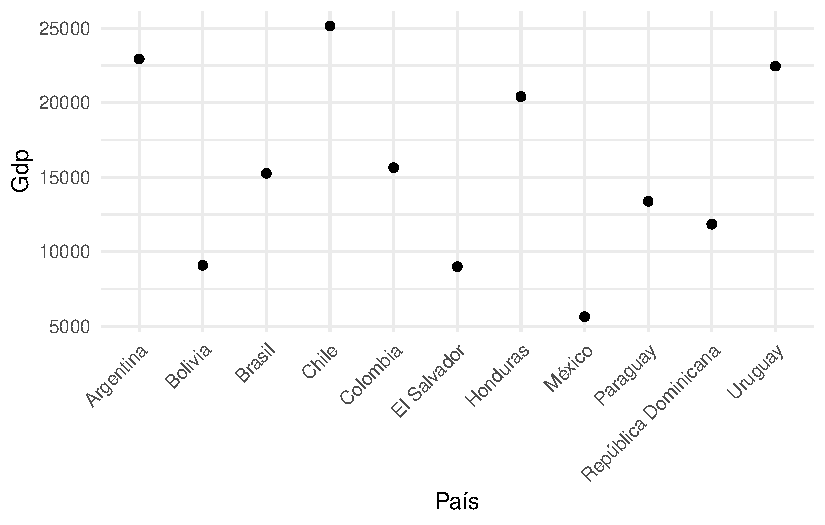
\includegraphics{taller-quarto-github_files/figure-pdf/fig-gdp-1.pdf}

}

\caption{\label{fig-gdp}Producto interno bruto por país}

\end{figure}%

Sin embargo la Figure~\ref{fig-gdp} entrega información desordenada.
Mejor ordenar por tamaño de PIB que por orden alfabético de los países.
Para eso

\begin{Shaded}
\begin{Highlighting}[]
\NormalTok{data\_sorted }\OtherTok{\textless{}{-}}\NormalTok{ data }\SpecialCharTok{\%\textgreater{}\%} \FunctionTok{arrange}\NormalTok{(}\FunctionTok{desc}\NormalTok{(gdp))}
\NormalTok{graph2}\OtherTok{\textless{}{-}}\FunctionTok{ggplot}\NormalTok{(data\_sorted, }\FunctionTok{aes}\NormalTok{(}\AttributeTok{x =} \FunctionTok{factor}\NormalTok{(idenpa, }\AttributeTok{levels =}\NormalTok{ idenpa), }\AttributeTok{y =}\NormalTok{ gdp)) }\SpecialCharTok{+}
  \FunctionTok{geom\_point}\NormalTok{() }\SpecialCharTok{+}
  \FunctionTok{labs}\NormalTok{(}\AttributeTok{x =} \StringTok{"País"}\NormalTok{, }\AttributeTok{y =} \StringTok{"GDP"}\NormalTok{) }\SpecialCharTok{+}
  \FunctionTok{theme\_minimal}\NormalTok{() }\SpecialCharTok{+}
  \FunctionTok{theme}\NormalTok{(}\AttributeTok{axis.text.x =} \FunctionTok{element\_text}\NormalTok{(}\AttributeTok{angle =} \DecValTok{45}\NormalTok{, }\AttributeTok{hjust =} \DecValTok{1}\NormalTok{))}

\NormalTok{graph2}
\end{Highlighting}
\end{Shaded}

\begin{figure}[H]

\centering{

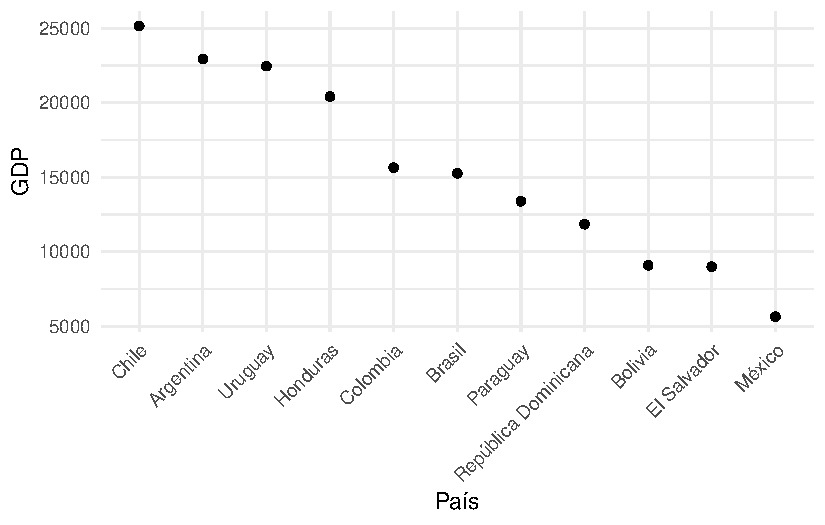
\includegraphics{taller-quarto-github_files/figure-pdf/fig-gdp-order-1.pdf}

}

\caption{\label{fig-gdp-order}Producto interno bruto por país ordenado}

\end{figure}%

Ahora sí la Figure~\ref{fig-gdp-order} muestra un gráfico más ordenado.

\subsubsection{Guardamos este nuevo gráfico en la carpeta
output}\label{guardamos-este-nuevo-gruxe1fico-en-la-carpeta-output}

\begin{Shaded}
\begin{Highlighting}[]
\FunctionTok{ggsave}\NormalTok{(graph2, }\AttributeTok{file=}\StringTok{"output/graphs/graph2.png"}\NormalTok{)}
\end{Highlighting}
\end{Shaded}

Y comparar el promedio de confianza en instituciones según producto
interno bruto por país?

\begin{Shaded}
\begin{Highlighting}[]
\NormalTok{data }\SpecialCharTok{\%\textgreater{}\%}
  \FunctionTok{ggplot}\NormalTok{(}\FunctionTok{aes}\NormalTok{(}\AttributeTok{x =}\NormalTok{ gdp, }\AttributeTok{y =}\NormalTok{ promedio, }\AttributeTok{label =}\NormalTok{ idenpa)) }\SpecialCharTok{+}
  \FunctionTok{geom\_point}\NormalTok{() }\SpecialCharTok{+}
  \FunctionTok{geom\_text}\NormalTok{(}\AttributeTok{vjust =} \SpecialCharTok{{-}}\FloatTok{0.5}\NormalTok{) }\SpecialCharTok{+}
  \FunctionTok{labs}\NormalTok{(}\AttributeTok{x =} \StringTok{"GDP"}\NormalTok{, }\AttributeTok{y =} \StringTok{"Promedio"}\NormalTok{) }\SpecialCharTok{+}
  \FunctionTok{theme\_bw}\NormalTok{()}
\end{Highlighting}
\end{Shaded}

\begin{figure}[H]

\centering{

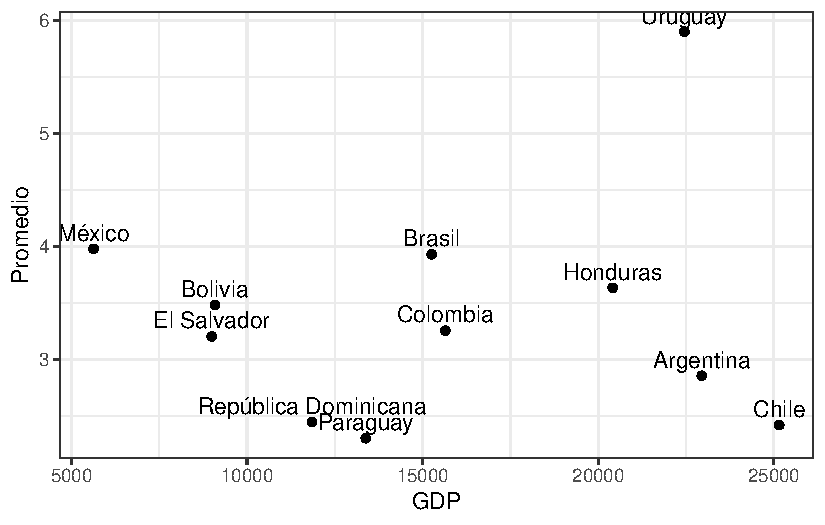
\includegraphics{taller-quarto-github_files/figure-pdf/fig-ctr-1.pdf}

}

\caption{\label{fig-ctr}Confianza en instituciones según el producto
interno bruto por país}

\end{figure}%

La Figure~\ref{fig-ctr} muestra la relación que existe entre el producto
interno bruto y la confianza en instituciones para los 18 países
analizados. Es interesante comparar los casos de Chile y urugay, que al
tener similar GDP, tienen un nivel de confianza en instituciones muy
diferente.

\begin{enumerate}
\def\labelenumi{\arabic{enumi}.}
\setcounter{enumi}{4}
\tightlist
\item
  Luego renderizamos
\end{enumerate}

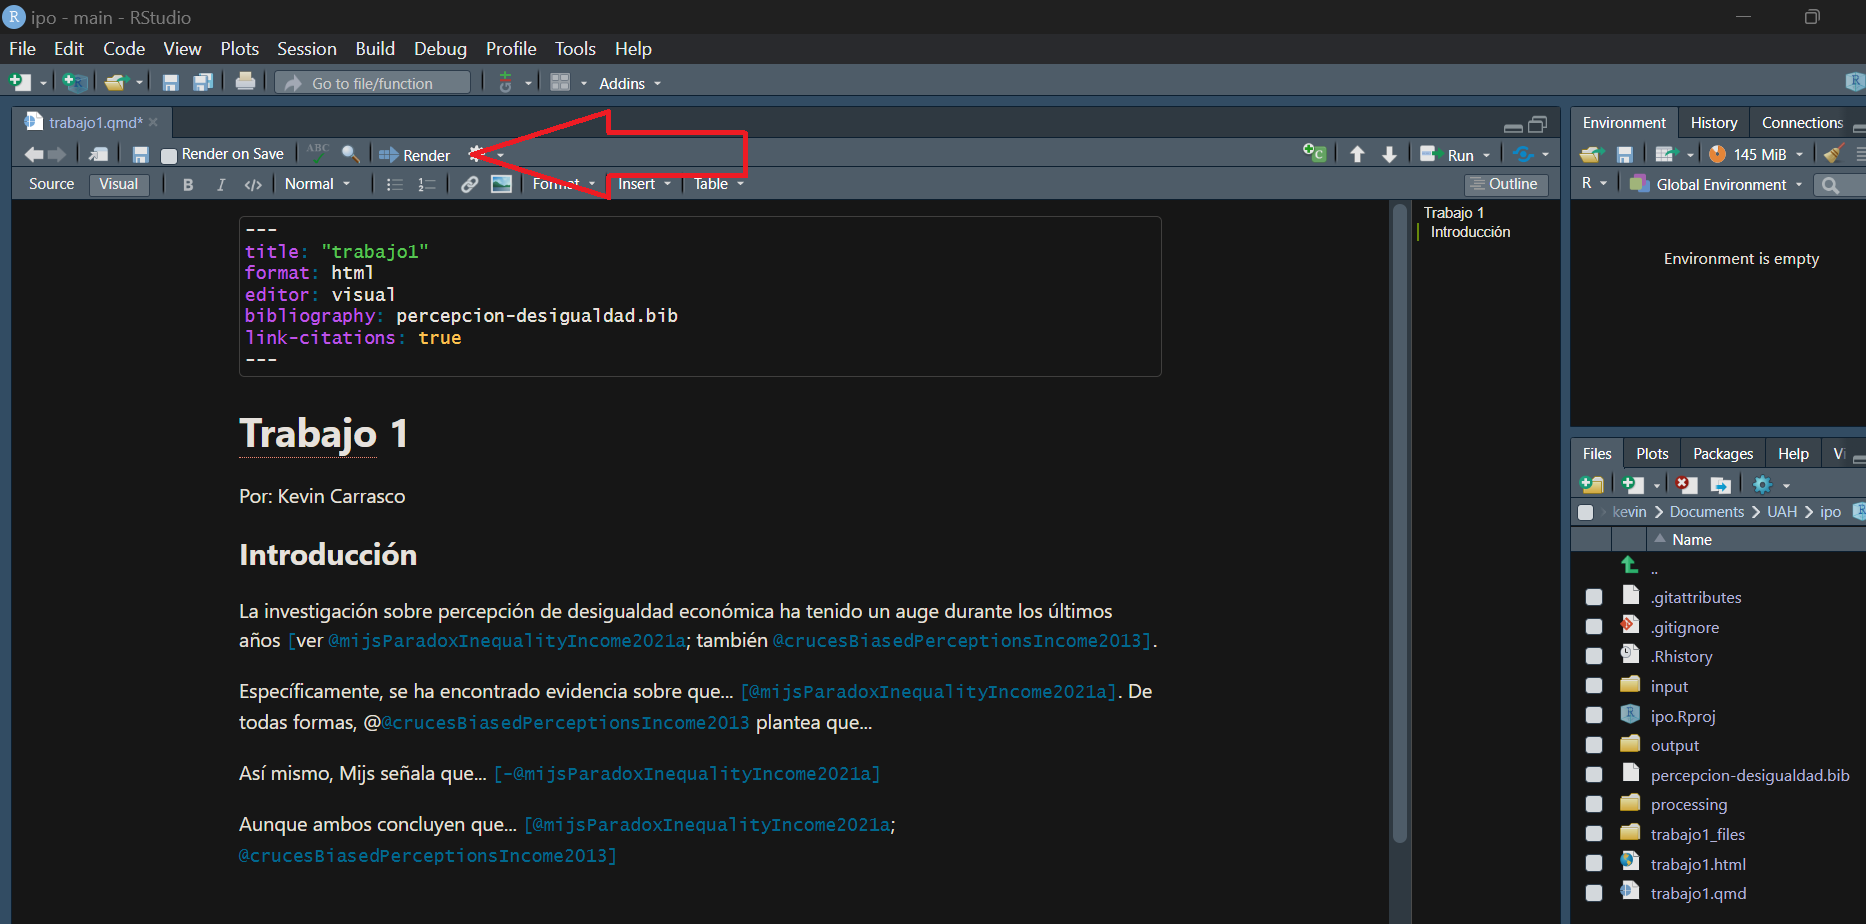
\includegraphics{images/quarto4.png}

y se debería ver así:

\begin{enumerate}
\def\labelenumi{\arabic{enumi}.}
\setcounter{enumi}{5}
\tightlist
\item
  Ahora que tenemos nuestra investigación podemos subirla a Github Pages
  a través de Github Desktop.
\end{enumerate}

\subsection{Github desktop}\label{github-desktop-1}

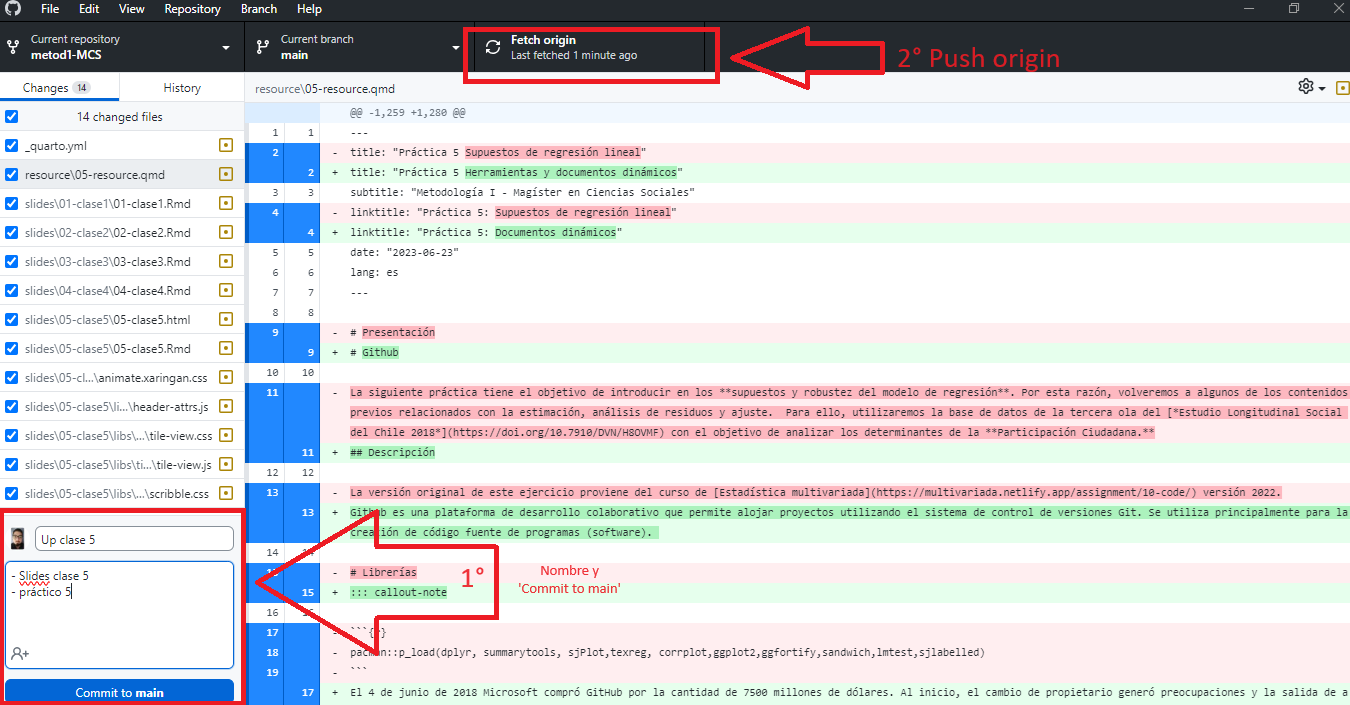
\includegraphics{images/push-github.png}

\subsection{Github pages}\label{github-pages}

Ahora podemos ver los documentos modificados en nuestro repositorio
online de github.

\begin{enumerate}
\def\labelenumi{\arabic{enumi}.}
\setcounter{enumi}{6}
\tightlist
\item
  Vamos a settings
\end{enumerate}

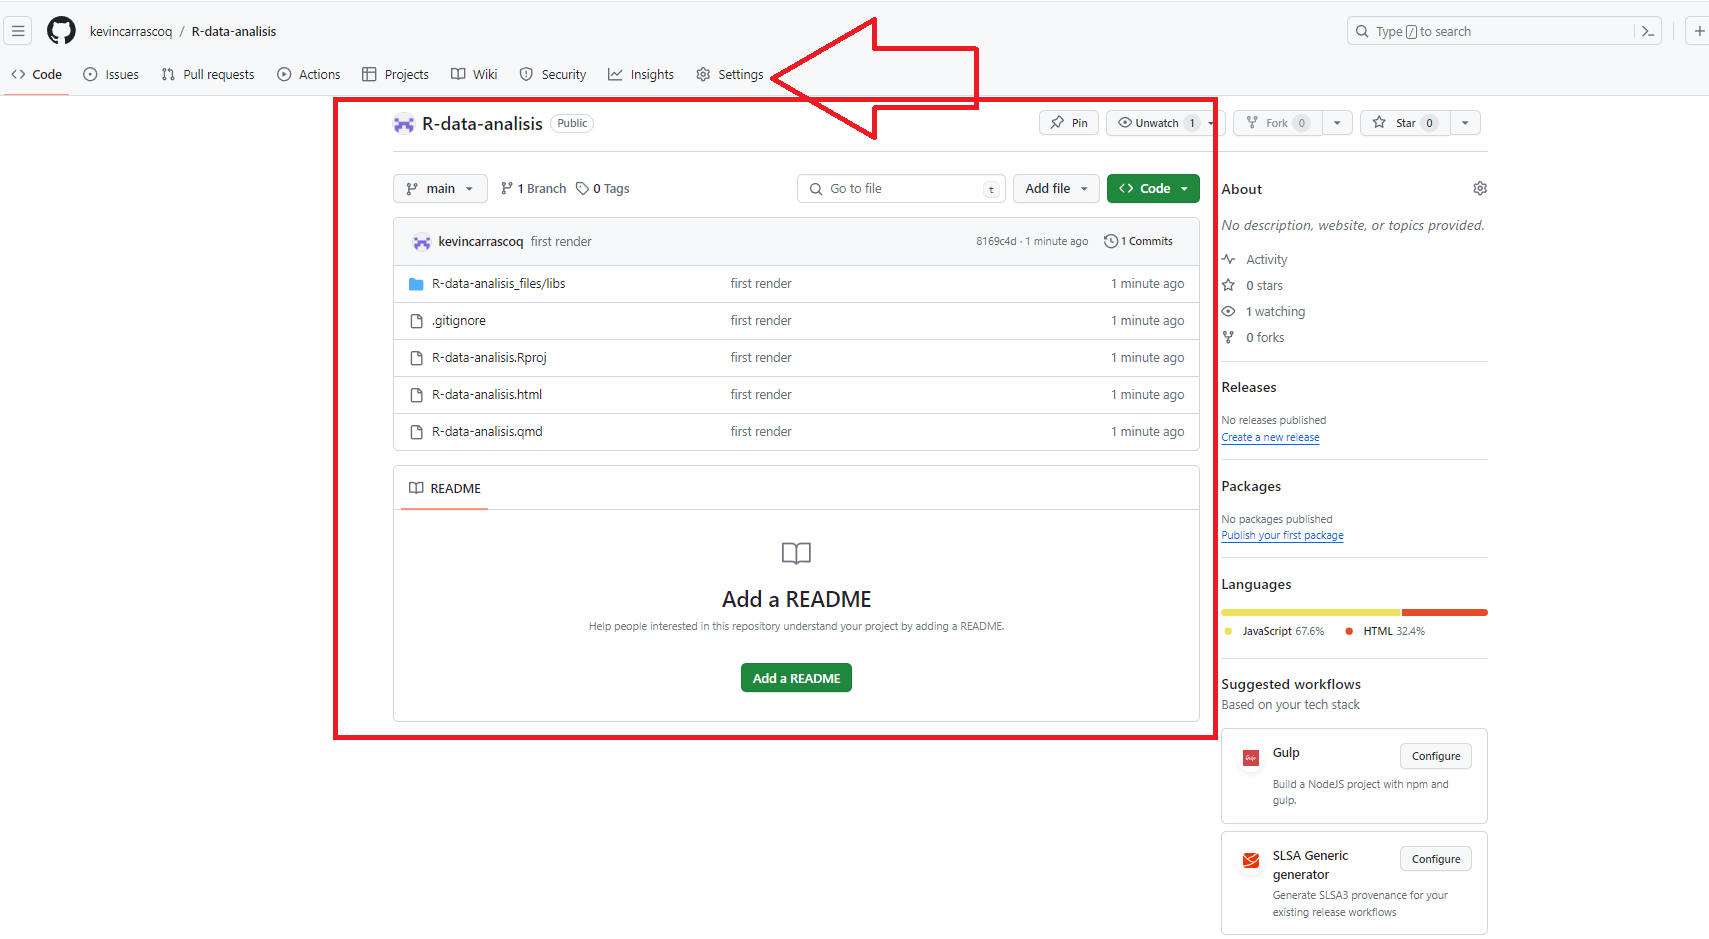
\includegraphics{images/pages.png}

\begin{enumerate}
\def\labelenumi{\arabic{enumi}.}
\setcounter{enumi}{7}
\tightlist
\item
  Dentro de Settings vamos a Pages, luego `none' y seleccionamos `main'.
  Luego apretamos Save
\end{enumerate}

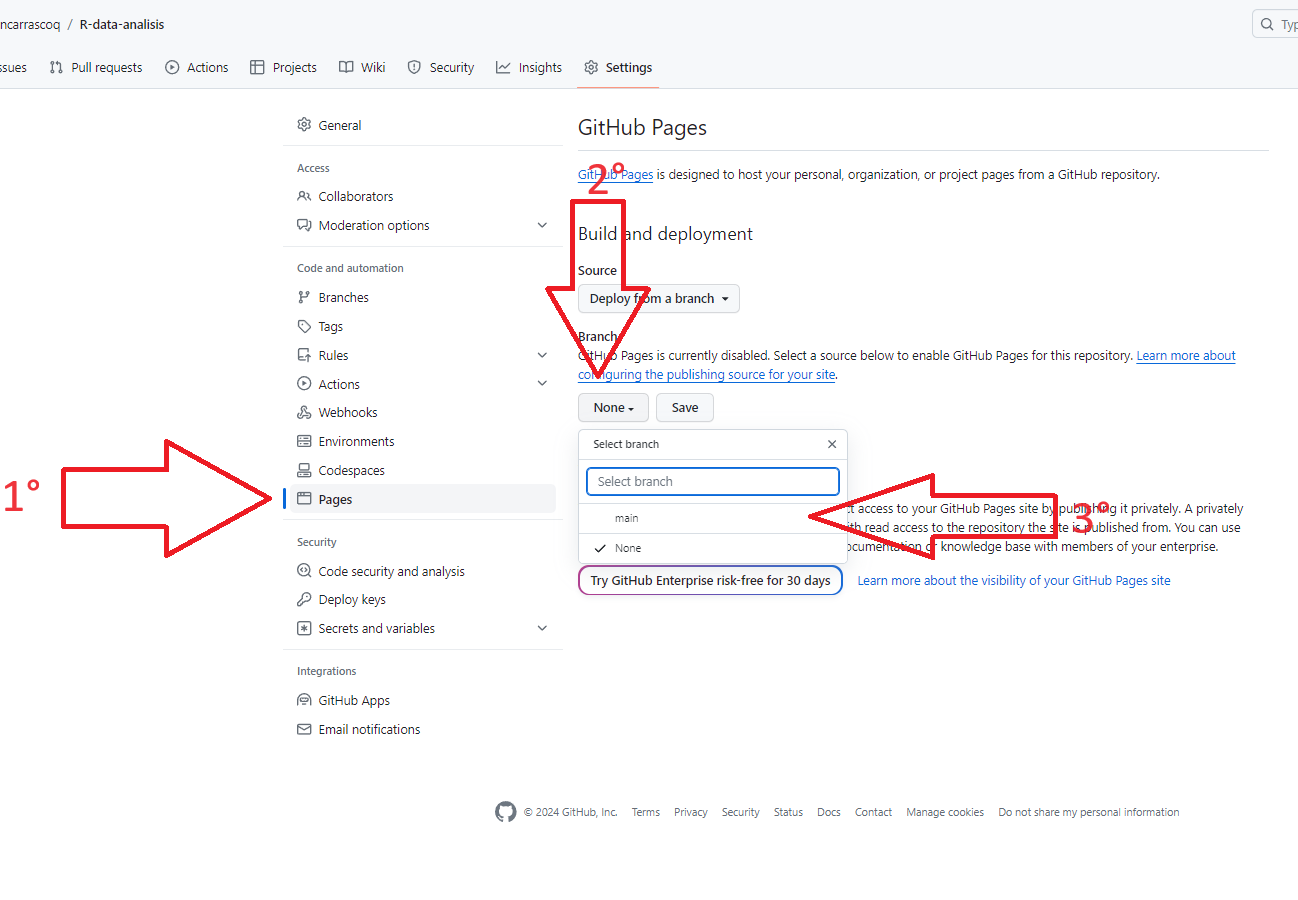
\includegraphics{images/pages2.png}

Luego de aproximadamente un minuto se actualiza la página y aparecerá un
link en la parte superior, algo así como
\url{kevin-carrasco.github.io/ipo} que es nuestra página principal de
nuestro sitio web de github.

El link para llegar a nuestro documento renderizado de quarto sigue la
estructura del repositorio:

kevin-carrasco.github.io/ipo/trabajo.html


\includegraphics{images/url-pages.png}




\end{document}
